\documentclass[preprint,5p,twocolumn,10pt,sort&compress]{elsarticle}

\usepackage{amssymb}
\usepackage{amsthm}
\setlength{\mathindent}{0pt}
\usepackage{tabularx}
\usepackage{graphicx}
\usepackage{epsfig}
\usepackage{textcomp}
\usepackage{subfigure}
\usepackage{natbib}
\usepackage[colorlinks,linkcolor=red,anchorcolor=yellow,citecolor=yellow]{hyperref}
\usepackage{color,soul}
\usepackage{multirow}
\usepackage{overpic}
\usepackage{amsmath}
\usepackage{caption}
\usepackage{bm}
\usepackage{framed}
\usepackage{threeparttable}
\usepackage{booktabs}
\usepackage{xeCJK}
% \usepackage{ctex}

\newcommand{\bfsigma}{{\mbox{\boldmath{$\sigma$}}}}
\newcommand{\bfepsilon}{{\mbox{\boldmath{$\varepsilon$}}}}
\newcommand{\dotbfepsilon}{{\mbox{\boldmath{$\dot\varepsilon$}}}}
\newcommand{\dotbfsigma}{{\mbox{\boldmath{$\dot\sigma$}}}}
\newcommand{\bftau}{{\mbox{\boldmath{$\tau$}}}}
\newcommand{\bfpsi}{{\mbox{\boldmath{$\psi$}}}}
\newcommand{\bfphi}{{\mbox{\boldmath{$\phi$}}}}
\newcommand{\bfalpha}{{\mbox{\boldmath{$\alpha$}}}}
\newcommand{\bfbeta}{{\mbox{\boldmath{$\beta$}}}}
\newcommand{\bfK}{{\bf K}}
\newcommand{\bff}{{\bf f}}
\newcommand{\bfn}{{\bf n}}
\newcommand{\bfm}{{\bf m}}
\newcommand{\bft}{{\bf t}}
\newcommand{\bfu}{{\bf u}}
\newcommand{\bfw}{{\bf w}}
\newcommand{\bfa}{{\bf a}}
\newcommand{\bfb}{{\bf b}}
\newcommand{\bfs}{{\bf s}}
\newcommand{\bfB}{{\bf B}}
\newcommand{\bfD}{{\bf D}}
\newcommand{\bfnabla}{{\mbox{\boldmath{$\nabla$}}}}
\newcommand{\bfDelta}{{\mbox{\boldmath{$\Delta$}}}}
\newcommand{\bfkappa}{{\mbox{\boldmath{$\kappa$}}}}
\newcommand{\bfN}{{\bf N}}
\newcommand{\bfT}{{\bf T}}
\newcommand{\bfG}{{\bf G}}
\newcommand{\bfH}{{\bf H}}
\newcommand{\dd}{{\rm d}}
\newcommand{\degreeC}{{$^\circ$C}}
\newcommand{\marked}[1]{\textcolor{red}{#1}}

\graphicspath{{figures/}}

\journal{International Journal of Fatigue}

\begin{document}

\captionsetup[figure]{labelfont={bf},font={footnotesize},name={Fig.},labelsep=period}

\captionsetup[table]{labelfont={bf},font={footnotesize},name={Table},labelsep=period}

\renewcommand\figureautorefname{Fig.}

\sethlcolor{yellow}

\begin{frontmatter}

%% Title, authors and addresses

%% use the tnoteref command within \title for footnotes;
%% use the tnotetext command for theassociated footnote;
%% use the fnref command within \author or \address for footnotes;
%% use the fntext command for theassociated footnote;
%% use the corref command within \author for corresponding author footnotes;
%% use the cortext command for theassociated footnote;
%% use the ead command for the email address,
%% and the form \ead[url] for the home page:
%% \title{Title\tnoteref{label1}}
%% \tnotetext[label1]{}
%% \author{Name\corref{cor1}\fnref{label2}}
%% \ead{email address}
%% \ead[url]{home page}
%% \fntext[label2]{}
%% \cortext[cor1]{}
%% \address{Address\fnref{label3}}
%% \fntext[label3]{}

\title{Life assessment of thermal gradient mechanical fatigue of a nickel-based superalloy Inconel 718}

%% use optional labels to link authors explicitly to addresses:
%% \author[label1,label2]{}
%% \address[label1]{}
%% \address[label2]{}

\author{Jingyu SUN}
\author{Huang YUAN\corref{cor1}}

\address{School of Aerospace Engineering, Tsinghua University, Beijing, China\fnref{label1}}
%\address[label2]{Department of Civil Engineering, Technical University of Darmstadt, Germany\fnref{label2}}
\cortext[cor1]{Corresponding author.}
\ead{yuan.huang@tsinghua.edu.cn}

\begin{abstract}
Turbine components generally work under thermomechanical  loading conditions  with varying temperature and significant thermal gradients. In the present work, a radiation heating system was developed to simulate thermal gradient mechanical fatigue (TGMF) loads in turbines. The specimen is externally heated by radiation and internally cooled by compressed air. Experiments showed that the TGMF life of the nickel-based superalloy is significantly shorter than that of  the thermomechanical and the isothermal fatigue, although the thermal stress amplitude related to the temperature gradient is small. It was confirmed that the conventional fatigue models generated seriously deviations and could not catch effects of the thermal gradients. The modified TGMF introduced  a correction term of the temperature gradient effects and can describe the TGMF lifetime of Inconel 718. The new model provides a uniform description of isothermal and complex thermomechanical fatigue. 
\end{abstract}

%\include{debut}
\begin{keyword}
% keywords here, in the form: keyword \sep keyword
Thermal gradient mechanical fatigue (TGMF) \sep transient temperature analysis \sep phase angle \sep nickel-based superalloy \sep fatigue life prediction

% PACS codes here, in the form: \PACS code \sep code
% \PACS
\end{keyword}
\end{frontmatter}

\section{Introduction}

The nickel-base superalloy Inconel 718 is widely used in the gas turbine engines \cite{Pollock2006}. In the past decades, isothermal fatigue (IF) tests were commonly used to predict the lifetime of the gas turbine components, which work generally under varying thermomechanical loading conditions. Numerous investigations on the elevated temperature LCF of the nickel-based superalloy were performed \cite{Koch85, Morrow88, Mahobia2014, Chen2016}. However, a number of studies showed that the thermomechanical fatigue (TMF) loads influenced the fatigue damage mechanisms significantly \cite{Evans2008, Bauer2009, Kulawinski2015, SCHLESINGER2017242, DENG2019813}. Thermomechanical fatigue means the mechanical loads and temperature are varying simultaneously. For different phases between the cyclic mechanical loading and temperature, the TMF lifetime can be shorter or longer than the isothermal one \cite{SUN2019228}.

The turbine blades are cooled by internal flow and the turbine discs are usually cooled by the secondary air system.
In the course of service, the turbine components are not only subjected to alternating  mechanical loads, but also to the impact of high temperature and the effect of cooling air on the surface and inside of the components, respectively. So the turbine parts suffer from thermomechanical fatigue damage caused by the varying loads and temperatures.
Moreover, the temperature gradient brings the multiaxial stress state to the parts and makes the fatigue multiaxial.
For internally cooled parts, the temperature gradient can produce additional stress, which is expressed as a multiaxial compressive load on the hotter surface, while a multiaxial tensile load is displayed on the colder surface.
Few works on the TGMF fatigue life were published.

Brendel et al. \cite{BRENDEL2008234} and Prasad et al. \cite{PRASAD2013131} investigated temperature gradients in TMF specimens. The results showed that the temperature gradients had the remarkable influence on the TMF lifetime.
Baufeld et al. \cite{BAUFELD2008219} and Bartsch et al. \cite{BARTSCH2008211} carried out the thermal gradient mechanical fatigue testing for the single-crystalline superalloy CMSX-4 with a NiPtAl oxidation protection coating.
Microstructural changes, defects, phase evolution of the metal coatings and rafting of the $\gamma$/$\gamma'$ substrate morphology were investigated. They detected the cracks at the inner specimen surface and substrate pores. However, the fatigue life of the TGMF was not studied. To quantify effects of temperature gradients in thermomechanical fatigue and to establish a uniform fatigue life prediction model for complex thermomechanical fatigue, extensive TGMF testing is necessary.

However, most published works on fatigue were performed in a standardized material testing systems, such MTS and INSTRON etc. Such test machines provide two typical heating systems: Silicon carbide heating elements and induction coils. The former is not suitable for transient varying temperature. 
The resistance furnace with the heating elements can reach a uniform temperature field in the furnace cavity. It has a high accuracy of homogeneous temperature and is widely used in isothermal tests, such as creep, low cycle fatigue, and creep-fatigue. However, the heating rate of the resistance furnace is slow and can not meet the requirement of rapid temperature varying in TMF testing. Additionally, the resistance furnace is an enclosed cavity, and it is difficult to perform forced air cooling of the specimen.

The induction heating has the advantages of high heating rate and high efficiency. It is widely used in TMF testing.
Due to the skin effect of the induced current, however, the induction heating usually only heats the surface of the specimen, and the higher the induction frequency, the shallower the heating depth. For thin-walled specimens with a thickness of  ca. 1 mm, the inner and outer surfaces of the specimen are heated simultaneously, which makes homogeneous temperature distribution in the thickness. Furthermore, considering a specimen covered with a thermal barrier coating (TBC), the induction heating can only heat the metallic substrate, and the TBC (typically a ceramic material) will not be heated. This will cause the temperature inside the specimen to be higher than the outside temperature, which does not meet the temperature distribution in actual working condition \cite{BRENDEL2008234}.  The TGMF test apparatus has not be standardized. 

Deutsches Zentrum f\"{u}r Luft- und Raumfahrt (DLR) \cite{BAUFELD2008219}  developed a thermal gradient mechanical fatigue (TGMF) test facilities which allow simultaneous cyclic thermal and mechanical loading with controlled thermal gradients over the wall of hollow specimens. 
The radiation heating is the use of quartz lamp to irradiate the specimen or workpiece to achieve the predetermined temperature field. Radiant heating can heat metals, non-metals, composites, etc., and can obtain complex temperature fields through multi-temperature zone control.
The thermal gradient is obtained by heating of the outer surface with a concentrating radiation furnace and simultaneous internal cooling with pressurized air. The high heat flux of the radiation furnace allows heating rates comparable to those in real turbine blades of a jet engine. The radiation furnace has a power of 16 kW and consists of 16 quartz lamps. A hollow cylindrical specimen from nickel base superalloy can be heated from 100$^\circ$C to 1000$^\circ$C in about 20 seconds. This design provides a new concept for the TGMF heating system.  

In the present work a radiation heating system is developed based on the DLR concept. Based on extensive finite element computations the transient temperature distributions in the thin-walled tubular specimens are optimized for thermal gradient mechanical fatigue tests. The numerical results are verified by experimental measurements and provide the basis for TGMF tests. LCF behavior of the nickel-based superalloy is experimentally tested under given both thermomechanical and thermal gradient mechanical loading conditions. The systematical experimental results provide a data base for assessing fatigue life models and for establishing new TGMF fatigue life concepts. 



\section{Experiments}

\subsection{Materials and specimens}
The nickel-based superalloy Inconel 718 investigated in the present paper was provided by ThyssenKrupp VDM GmbH, in the form of rods of the 20 mm diameter.
The rods were solution-treated at 980$^{\circ}$C for one and a half hours then cooled to room temperature in water.
Then they were exposed for eight hours at 720$^{\circ}$C, furnace cooled at 56$^{\circ}$C/h to 621$^{\circ}$C, where they were held for eight hours and forced air cooling to room temperature.
The chemical compositions of Inconel 718 are given in Table \ref{Tab:ChemicalCompositionofIN718}.
The average grain size is about 20 $\rm{\mu }$m.

\begin{table}[!ht]
  \centering
  \caption{Chemical compositions of  Inconel 718 (wt. \%)}
    \begin{tabular}{llll}
    \toprule
    Element & wt. \% & Element & wt. \% \\
    \midrule
    C     & 0.02  & Fe    & 17.71 \\
    S     & $<$0.001 & P     & 0.007 \\
    Cr    & 18.53 & Al    & 0.56 \\
    Ni    & 53.44 & Pb    & 0.0002 \\
    Mn    & 0.05  & Co    & 0.13 \\
    Si    & 0.06  & B     & 0.004 \\
    Mo    & 3.06  & Ta    & $<$0.01 \\
    Ti    & 0.99  & Se    & $<$0.0003 \\
    Nb    & 5.30  & Bi    & $<$0.00003 \\
    Cu    & 0.04  &       &  \\
    \bottomrule
    \end{tabular}%
  \label{Tab:ChemicalCompositionofIN718}
\end{table}

%\subsection{Specimen}
Fatigue testing specimens were in the thin-walled tubular shape. The geometry of the thin-walled tubular specimen is shown in \autoref{Fig:IN718_Axial_Specimen_TGMF}, with 120 mm in the total length, a gauge length of 30 mm, an outer diameter of the gauge section of 8.5 mm and an inner diameter of 6.5 mm. Thus, the wall thickness of the tubular specimen in the gauge section is 1 mm. All specimens were manufactured in a CNC machining center, and the surfaces were polished. 

\begin{figure}[!ht]
\centering{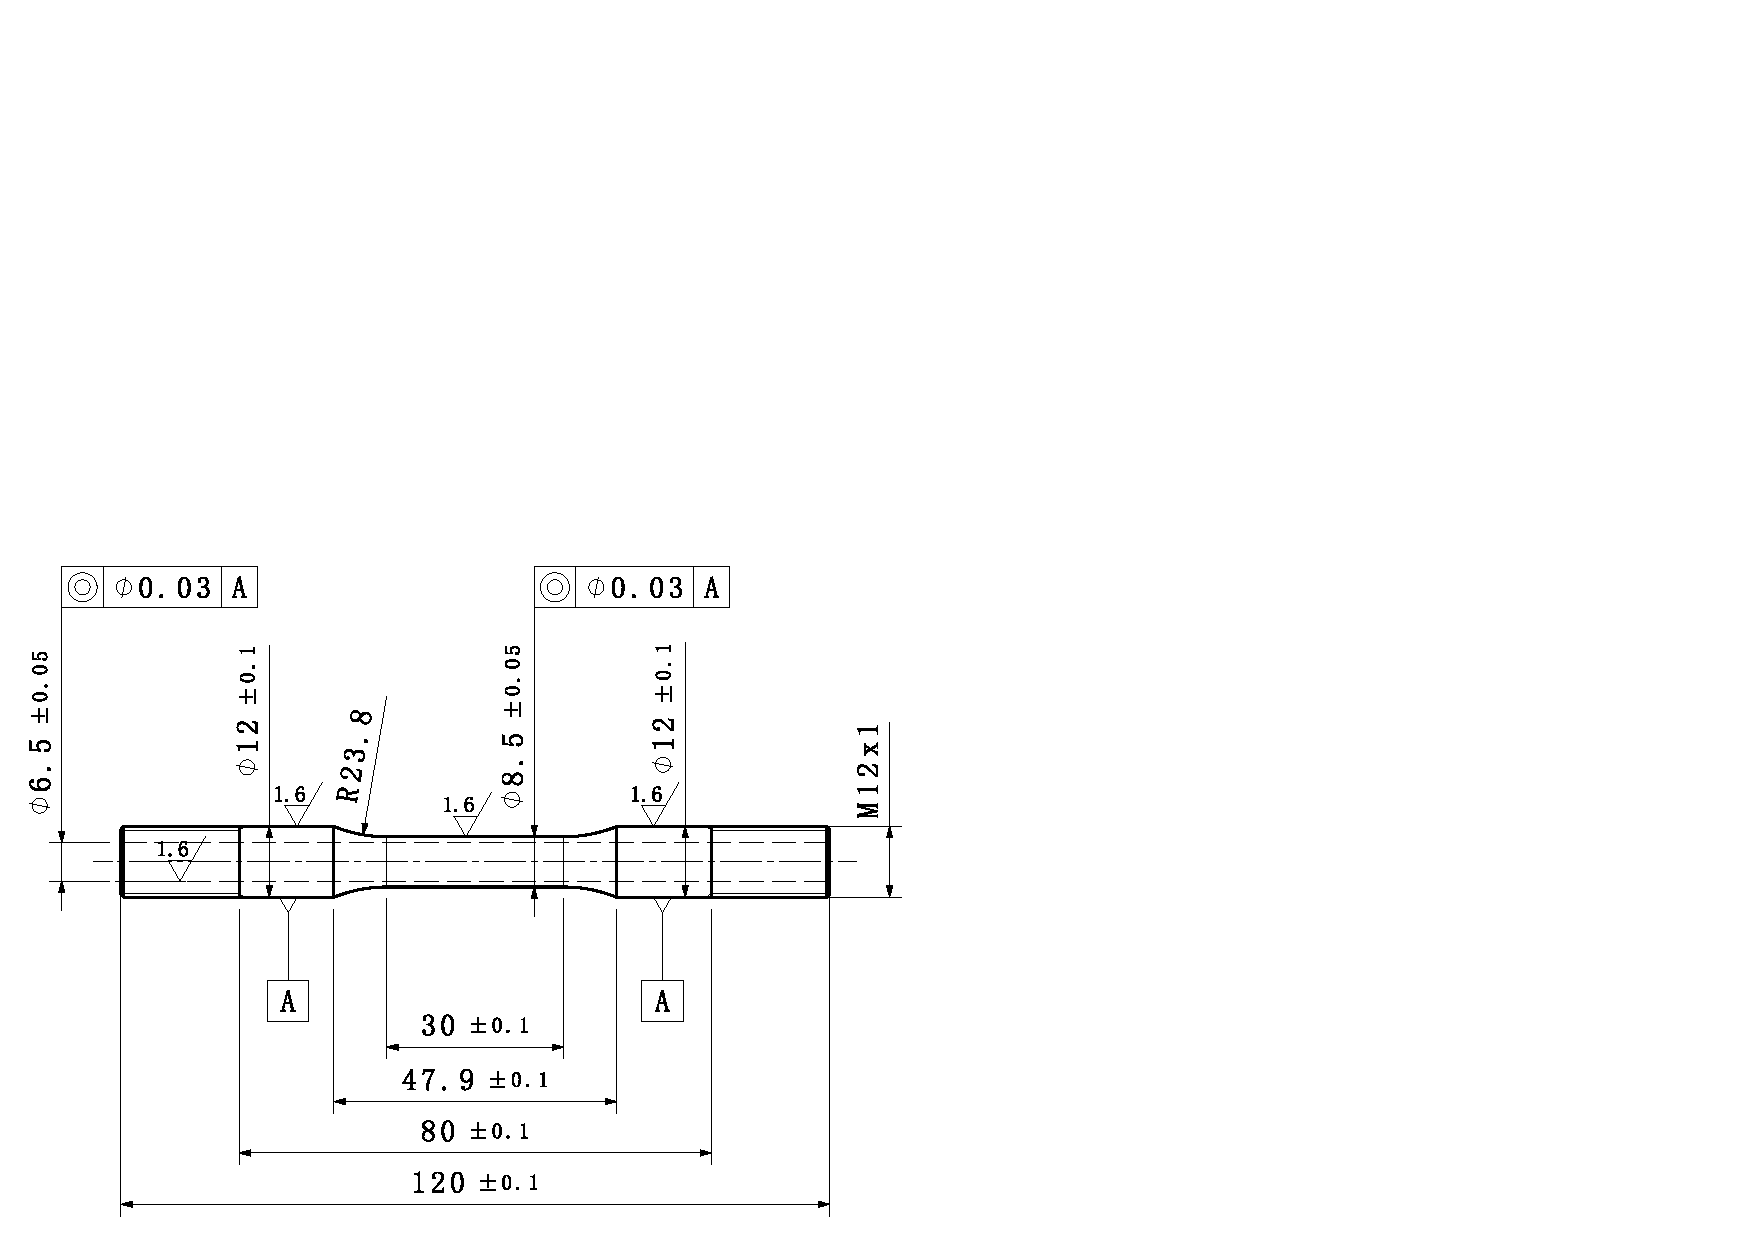
\includegraphics[width=7.5cm]{IN718_Axial_Specimen_TGMF.pdf}}
\caption{Dimensions of the specimen for TGMF testing.}
\label{Fig:IN718_Axial_Specimen_TGMF}
\end{figure}

\subsection{TGMF testing system}
The thermal gradient mechanical fatigue (TGMF) testing system for the thin-walled tubular specimen was developed, as shown in \autoref{Fig:tgmf_testing}. The specimen in the TGMF tests were heated by focused radiation heating from quartz lamps. Radiant heating can heat metals, non-metals, composites, etc., and can obtain complex temperature fields through multi-temperature zone control \autoref{Fig:cooling}. The total power of the radiation furnace is 6.4 kW and can heat the tubular specimens to melt within seconds.
The system includes multiple subsystems such as loading, heating, air cooling, and water cooling. These subsystems work cooperatively to ensure the mechanical load and temperature over the specimen gauge section are simultaneously varied and independently controlled. 
\begin{figure}[!ht]
\centering{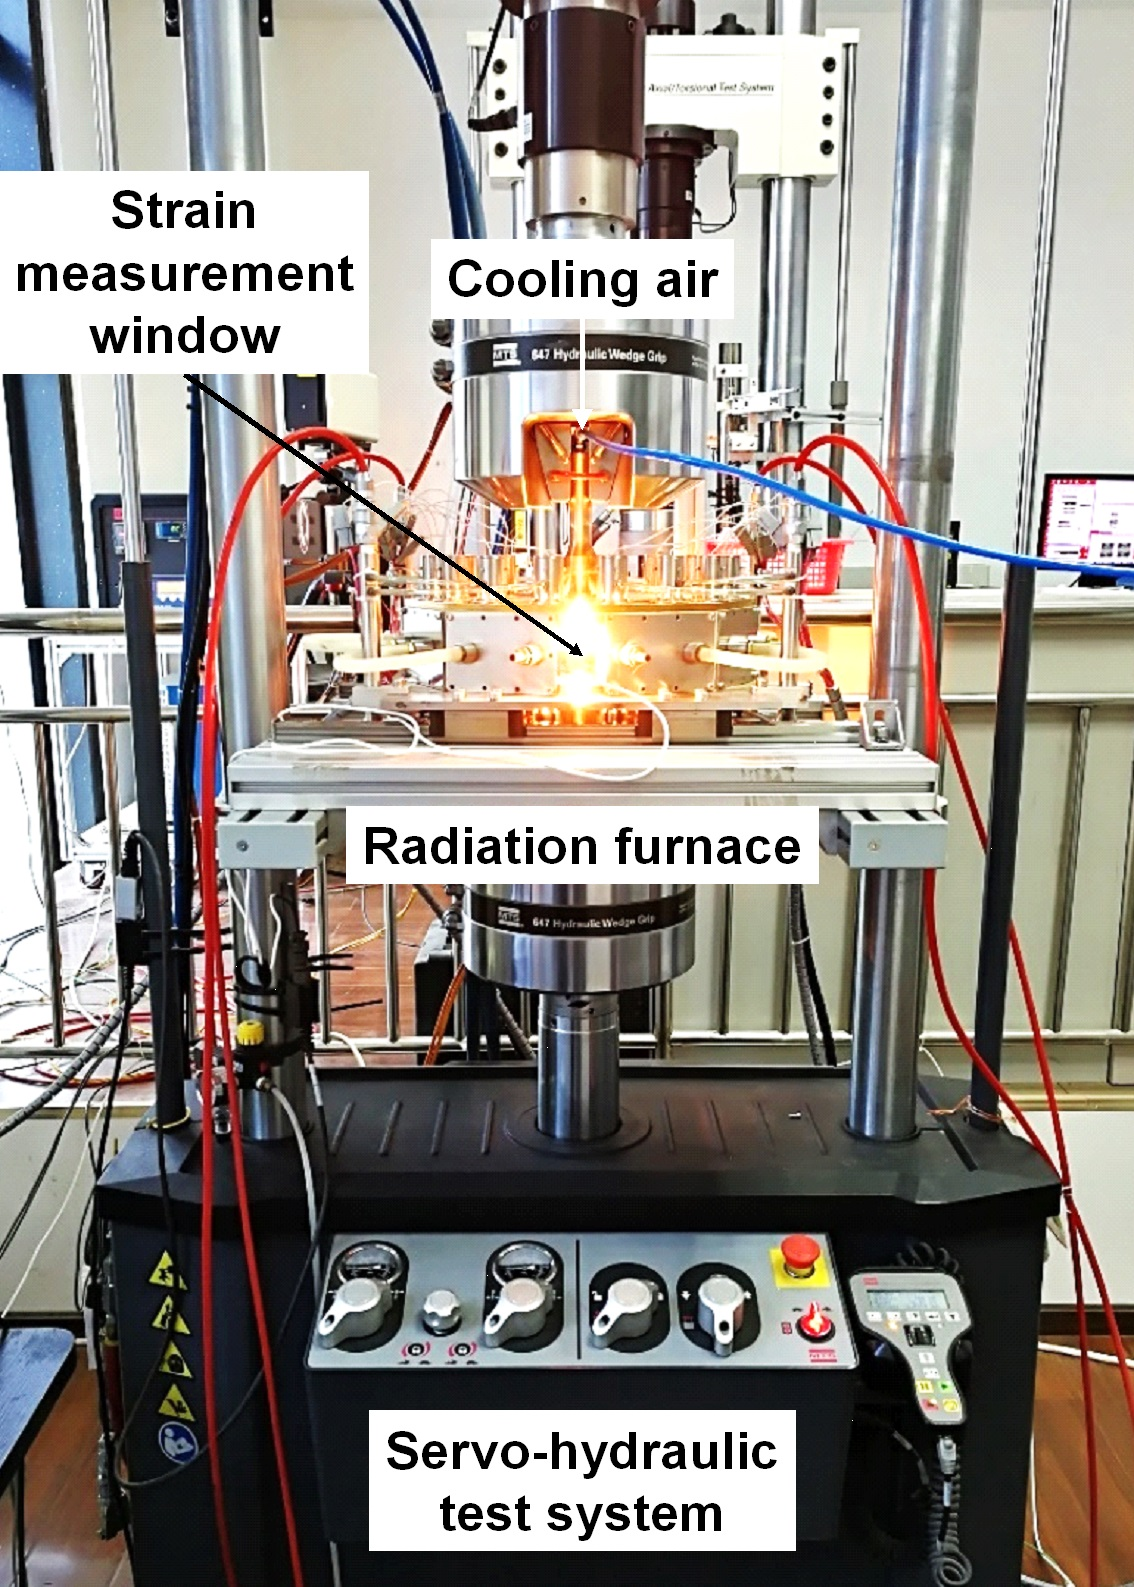
\includegraphics[height=10.0cm]{tgmf_testing.jpg}}
\caption{Experimental apparatus of TGMF test system.}
\label{Fig:tgmf_testing}
\end{figure}

A MTS hydraulic servo fatigue test machine was used to apply a tension/compression mechanical load. The mechanical load is transmitted to the specimen through a fixture. As shown in \autoref{Fig:cooling}, the cooling air can enter the internal of the tubular specimen through the fixture. In order to reduce the additional bending moments and the bending stress in the specimen, the fixture must provide a sufficiently high degree of coaxiality. Meanwhile, the frame of the MTS testing system provides an alignment device, and it can effectively reduce the additional bending moments in the specimen during the test. The total strain is measured by an extensometer with a gauge length of 10 mm and a measuring range of $\pm$20\%. 

\begin{figure}[!ht]
	\centering
	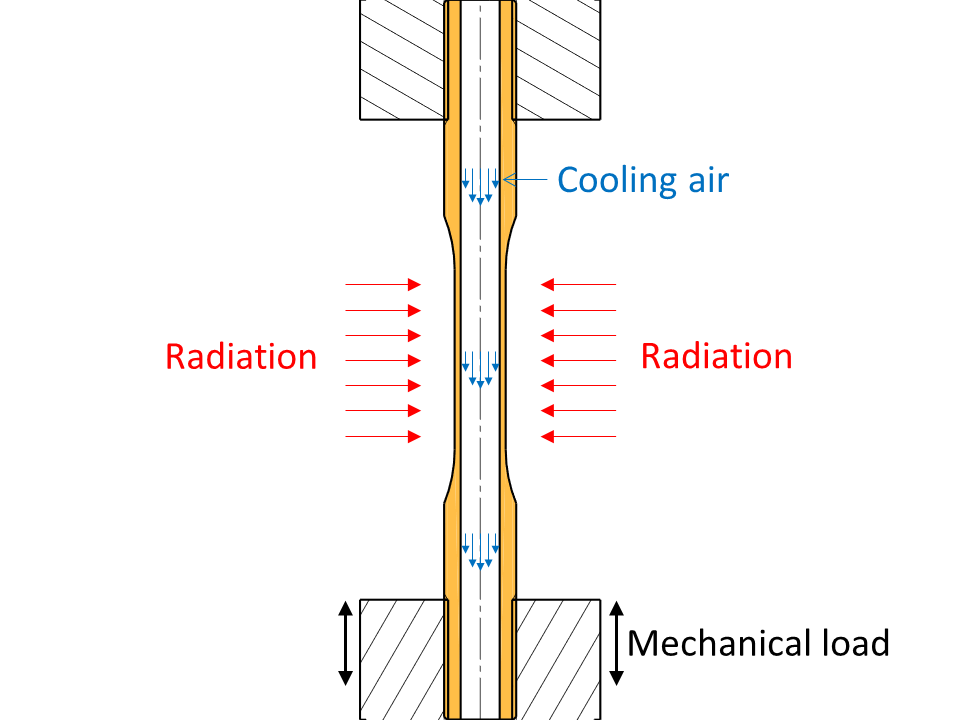
\includegraphics[width=7.5cm]{cooling.png}
	\caption{Principle of the TGMF radiation furnace with temperature monitors.}
	\label{Fig:cooling}
\end{figure}

The temperature of the specimen was measured by the thermocouples. In practice, the choice of the diameter of the thermocouple wire is significant. A thick thermocouple  will cause a delay in the temperature measurement. It leads to a temperature deviation between the thermocouple and the specimen, and it affects the response of the feedback control system. In order to improve the accuracy of temperature measurement and increase the response speed of thermocouples, the diameter of the thermocouple should be as small as possible. Therefore, the thermocouple with a diameter of 0.25 mm was used.

The temperature controller was used to control the temperature of the specimen.
The controller accepted the temperature sensor (thermocouple or infrared thermometer) as input and compared the actual temperature with the desired temperature. It then provided an output to the power regulator to control the luminance of the lamps, i.e. the heat power of the specimen. 
The temperature controller of the radiation furnace is a proportional-integral-derivative (PID) controller. The values of proportional, integral, and derivative gains of the PID controller can be determined by the PID tuning process.
However, the emissivity of the specimen and the temperature range influence the PID gains of the temperature controller. Therefore, the PID gains should be tuned when the specimen surface was fully oxidized.

The air cooling subsystem consists of two air compressors, an air dryer, metering valves, air pressure gauges and cooling passages. 
The two air compressors were used to provide the cooling air of the specimen and the lamp holders, separately.
Each air compressor has a power of 2.4 kW and provides the compressed air of 0.4 - 0.8 MPa. The compressed air with a pressure of 0.7 MPa is filtered through the air dryer and output to the metering valve. The air dryer is used for removing water vapor from the compressed air.
During all of the TGMF tests, the pressure and the flow volume  of the compressed air were kept as constant to 40 l/min. The metering valve was used to control the volume flow of the compressed air.
The air cooling subsystem also provides compressed air for the lamp holders.
The duration of the TGMF test is usually long, so the lamp holders have to be cooled to ensure that they can work properly.


There are no relevant standards for TGMF testing. Since the test processes of the TGMF and TMF are very similar,  the concepts in TGMF testing are defined as same as those of the TMF testing, such as:
\begin{itemize}
  \item {Thermal strain}, $\varepsilon_{\rm{th}}$,
  \item {Mechanical strain}, $\varepsilon_{\rm{mech}}$,
  \item {Total strain}, $\varepsilon_{\rm{tot}}=\varepsilon_{\rm{mech}}+\varepsilon_{\rm{th}}$,
  \item {Loading ratio}, $R_{\varepsilon}=\varepsilon_{\rm{mech,min}}/\varepsilon_{\rm{mech,max}}$,
  \item {Phase angle of the thermal loading and mechanical loading}, $\theta_{T-\varepsilon}$.
\end{itemize}

\begin{figure}[!ht]
	\centering
	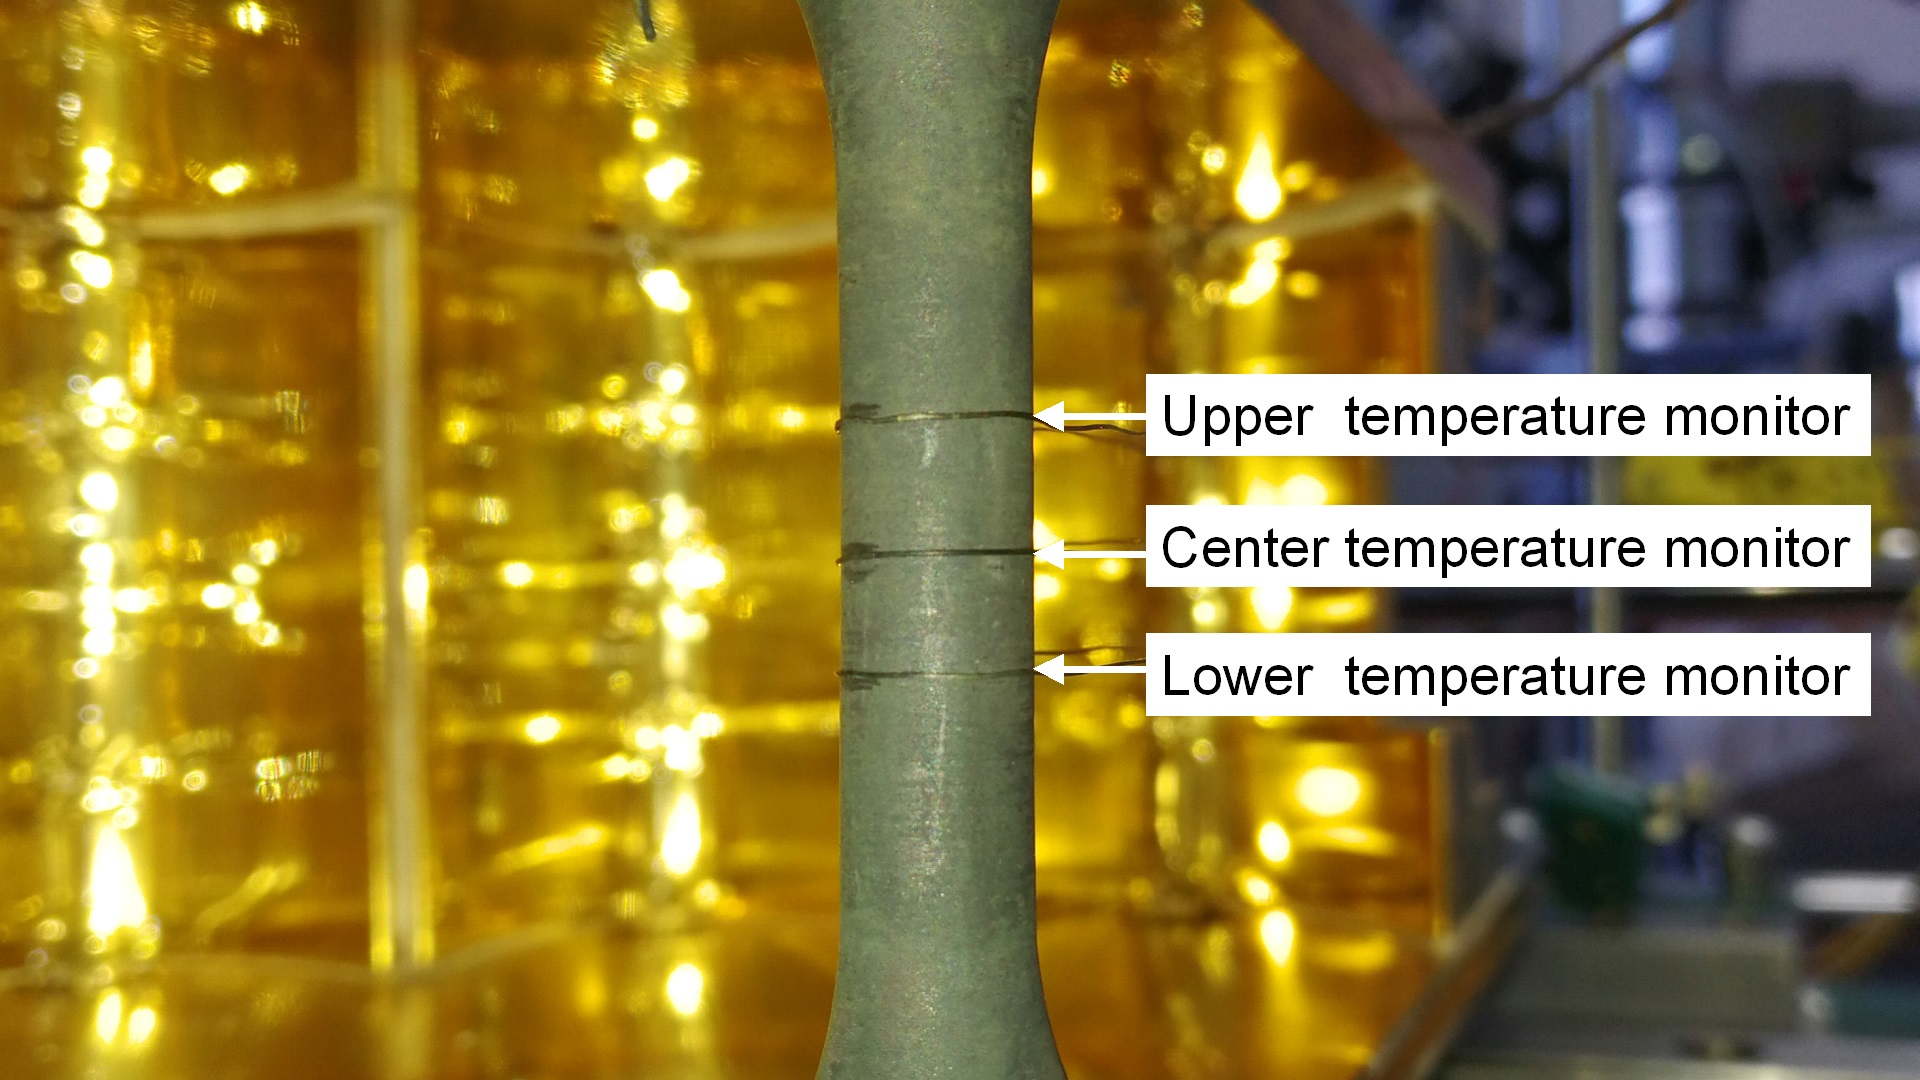
\includegraphics[width=7.5cm]{temperature_monitors_tgmf.jpg}
	\caption{Locations of the temperature monitors.}
	\label{Fig:temperature_monitors_tgmf}
\end{figure}



\begin{figure}[!ht]
	\centering
	\begin{overpic}[width=7.5cm]{plot_thermal_stability_tgmf.pdf}
		\put(84,65){\fcolorbox{white}{white}{(a)}}
	\end{overpic}
	\begin{overpic}[width=7.5cm]{plot_thermal_stability_tgmf_deviation.pdf}
		\put(84,65){\fcolorbox{white}{white}{(b)}}
	\end{overpic}
	\caption{Varying temperatures in a tubular specimen with the gauge length of 15 mm, heated by the radiation furnace. (a) Temperature variations of three thermal elements during a loading cycle. (b) Temperature deviations in the axial direction.}
	\label{Fig:thermal_stability_TGMF}
\end{figure}

The light reflected on the different gold-coated mirrors focuses on the specimen and induces temperature gradients along the specimen outer surface. The highest temperature occurs at the middle section of the specimen during the TGMF test.
Unlike the induction heating, the axial temperature gradient of the specimen is difficult to adjust by modifying the radiation furnace.
Therefore, the influence of the axial temperature gradients has to be considered in the computation.

In order to obtain the temperature distribution of the specimen during the TGMF testing, temperatures at the upper, center and lower positions in the 12 mm gauge section of the specimen were measured by three thermocouples wrapped around the specimen. \autoref{Fig:temperature_monitors_tgmf} shows the locations of the thermocouples. In the present work, the temperature of the TGMF testing varies between 300$^\circ$C and 650$^\circ$C. The cycle period was predetermined as 240 s with a triangular shape temperature cycle, thus the heating and cooling rates were about 2.2$^\circ$C/s.
\autoref{Fig:thermal_stability_TGMF}(a) shows the transient temperature measurement during a TGMF cycle and \autoref{Fig:thermal_stability_TGMF}(b) shows the temperature deviations between upper/lower thermocouple and the temperature command.
The maximum axial temperature difference during the TMF test are less than $\pm30$$^\circ$C. The deviations in the center of the specimen, where the fatigue failure occurs, are obviously smaller, less than $\pm 10^\circ$C. 


\section{Results of TGMF tests}

The experimental conditions and results of thermo-mechanical fatigue tests are summarized in \autoref{Tab:test_matrix_TGMF}. The isothermal fatigue (IF) tests were performed at 650$^\circ$C, and the in-phase thermo-mechanical fatigue (TMF-IP) and the out-of-phase thermo-mechanical fatigue (TMF-OP) tests were carried out with a temperature range of 300$\sim$650$^\circ$C, as introduced in \cite{SUN2019228, SUN201989}. In order to compare with the TMF testing results, the TGMF tests with the same temperature range of 300$\sim$650$^\circ$C and two kinds of phase angles were carried out: 0$^\circ$ (IP) and 180$^\circ$ (OP). Each kind of TGMF tests was conducted with four or five different mechanical strain amplitudes. The load type TGMF-IP stands for the in-phase thermal gradient mechanical fatigue, and TGMF-OP means the out-of-phase thermal gradient mechanical fatigue. The nickle-based superalloy Inconel 718 used in  \cite{SUN2019228, SUN201989} were investigated in the present work under the TGMF loading conditions, therefore, it is reasonable to compare the fatigue lifetime of those tests.

Because of the thermal gradients in radial and axial directions, the axial stress is not constant on the cross-section of the specimen.
Therefore, the stress distribution of the specimen during the test has to be obtained by the finite element method computation.
In order to facilitate the comparison and analysis between the computational and experimental results, the nominal axial stress $\sigma$ on the cross section is used in the following figures, defined as
\begin{equation}
\sigma = F/A.
\end{equation}
Figs. \ref{Fig:plot_exp_TCTGMF}(a) and (c) show the stable hysteresis loops of TGMF tests under IP and OP loading conditions, respectively.
Since there is a phase difference between the temperature cycle and the load cycle in the fatigue test, the tensile half cycle and the compressive half cycle have different cycle softening behaviors.
For the TGMF-IP test, an evident cyclic softening was observed during the tensile half cycle, whereas for the TGMF-OP test, the alloy performed a significant cyclic softening during the compressive half cycle.

% 如果是右对齐,那么只需要将\centering换成\raggedleft,如果左对齐,那么换成\raggedright即可。
\begin{table}[!ht]
  \centering
  \caption{Experimental conditions and results of thermal gradient mechanical fatigue tests.}
    \begin{tabular}{p{2.0cm}p{1.0cm}<{\centering}p{2cm}<{\centering}p{0.6cm}<{\centering}p{1.2cm}<{\raggedleft}}
    \toprule
    Test Type & $\pm \varepsilon _{\rm{mech}}$ & $\dot \varepsilon _{\rm{mech}}$ & $\theta_{\rm{T-\varepsilon}}$ & $N_{\rm{f}}$ \\
          & [\%]  & [s$^{-1}$] & [$^\circ$] & [cycle] \\
    \midrule
    IF \cite{SUN2019228} & 1.00  & $1\times 10^{-3}$ & -  & 231 \\
          & 0.80  & $1\times 10^{-3}$ & -  & 326 \\
          & 0.70  & $1\times 10^{-3}$ & -  & 592 \\
          & 0.60  & $1\times 10^{-3}$ & -  & 1336 \\
          & 0.50  & $1\times 10^{-3}$ & -  & 8449 \\
          & 0.45  & $1\times 10^{-3}$ & -  & 15497 \\
          & 0.40  & $6.4\times 10^{-3}$ & -  & 130585 \\
    \midrule
    TMF-IP  & 1.00 & $2.22\times 10^{-4}$ & 0   & 58 \\
    \cite{SUN2019228}      & 0.80 & $1.78\times 10^{-4}$ & 0   & 176 \\
          & 0.70 & $1.56\times 10^{-4}$ & 0   & 248 \\
          & 0.60 & $1.33\times 10^{-4}$ & 0   & 1297 \\
    \midrule
    TMF-OP  & 1.00 & $2.22\times 10^{-4}$ & 180 & 209 \\
    \cite{SUN2019228}      & 0.80 & $1.78\times 10^{-4}$ & 180 & 303 \\
          & 0.70 & $1.56\times 10^{-4}$ & 180 & 429 \\
          & 0.65 & $1.44\times 10^{-4}$ & 180 & 633 \\
    \midrule
    TGMF-IP & 0.80  & $1.67\times 10^{-4}$ & 0     & 48 \\
          & 0.70  & $1.33\times 10^{-4}$ & 0     & 50 \\
          & 0.60  & $1.22\times 10^{-4}$ & 0     & 107 \\
          & 0.50  & $1.11\times 10^{-4}$ & 0     & 208 \\
          & 0.425  & $0.89\times 10^{-4}$ & 0     & 1066 \\
    \midrule
    TGMF-OP & 0.80  & $1.67\times 10^{-4}$ & 180   & 128 \\
          & 0.60  & $1.22\times 10^{-4}$ & 180   & 375 \\
          & 0.50  & $1.11\times 10^{-4}$ & 180   & 864 \\
          & 0.425  & $0.89\times 10^{-4}$ & 180   & 3387 \\
    \bottomrule
    \end{tabular}%
  \label{Tab:test_matrix_TGMF}%
\end{table}%

\begin{figure*}[!ht]
  \centering
  \begin{overpic}[width=7.5cm]{plot_exp_half_life_cycle_TCIPTGMF.pdf}
    \put(84,13){\fcolorbox{white}{white}{(a)}}
  \end{overpic}
  \begin{overpic}[width=7.5cm]{plot_exp_pv_TCIPTGMF.pdf}
    \put(84,13){\fcolorbox{white}{white}{(b)}}
  \end{overpic}

  \begin{overpic}[width=7.5cm]{plot_exp_half_life_cycle_TCOPTGMF.pdf}
    \put(84,13){\fcolorbox{white}{white}{(c)}}
  \end{overpic}
  \begin{overpic}[width=7.5cm]{plot_exp_pv_TCOPTGMF.pdf}
    \put(84,13){\fcolorbox{white}{white}{(d)}}
  \end{overpic}

  \caption{Experimental results of TGMF tests with varying temperature between 300$^\circ$C and 650$^\circ$C. Noting that, the vertical axis axial stress $\sigma$ is the nominal stress.
  (a) Half life stable hysteresis loops of TGMF-IP tests.
  (b) Peak and valley stresses of TGMF-IP tests.
  (c) Half life stable hysteresis loops of TGMF-OP tests.
  (d) Peak and valley stresses of TGMF-OP tests.}
  \label{Fig:plot_exp_TCTGMF}
\end{figure*}

\begin{figure}[!ht]
  \centering{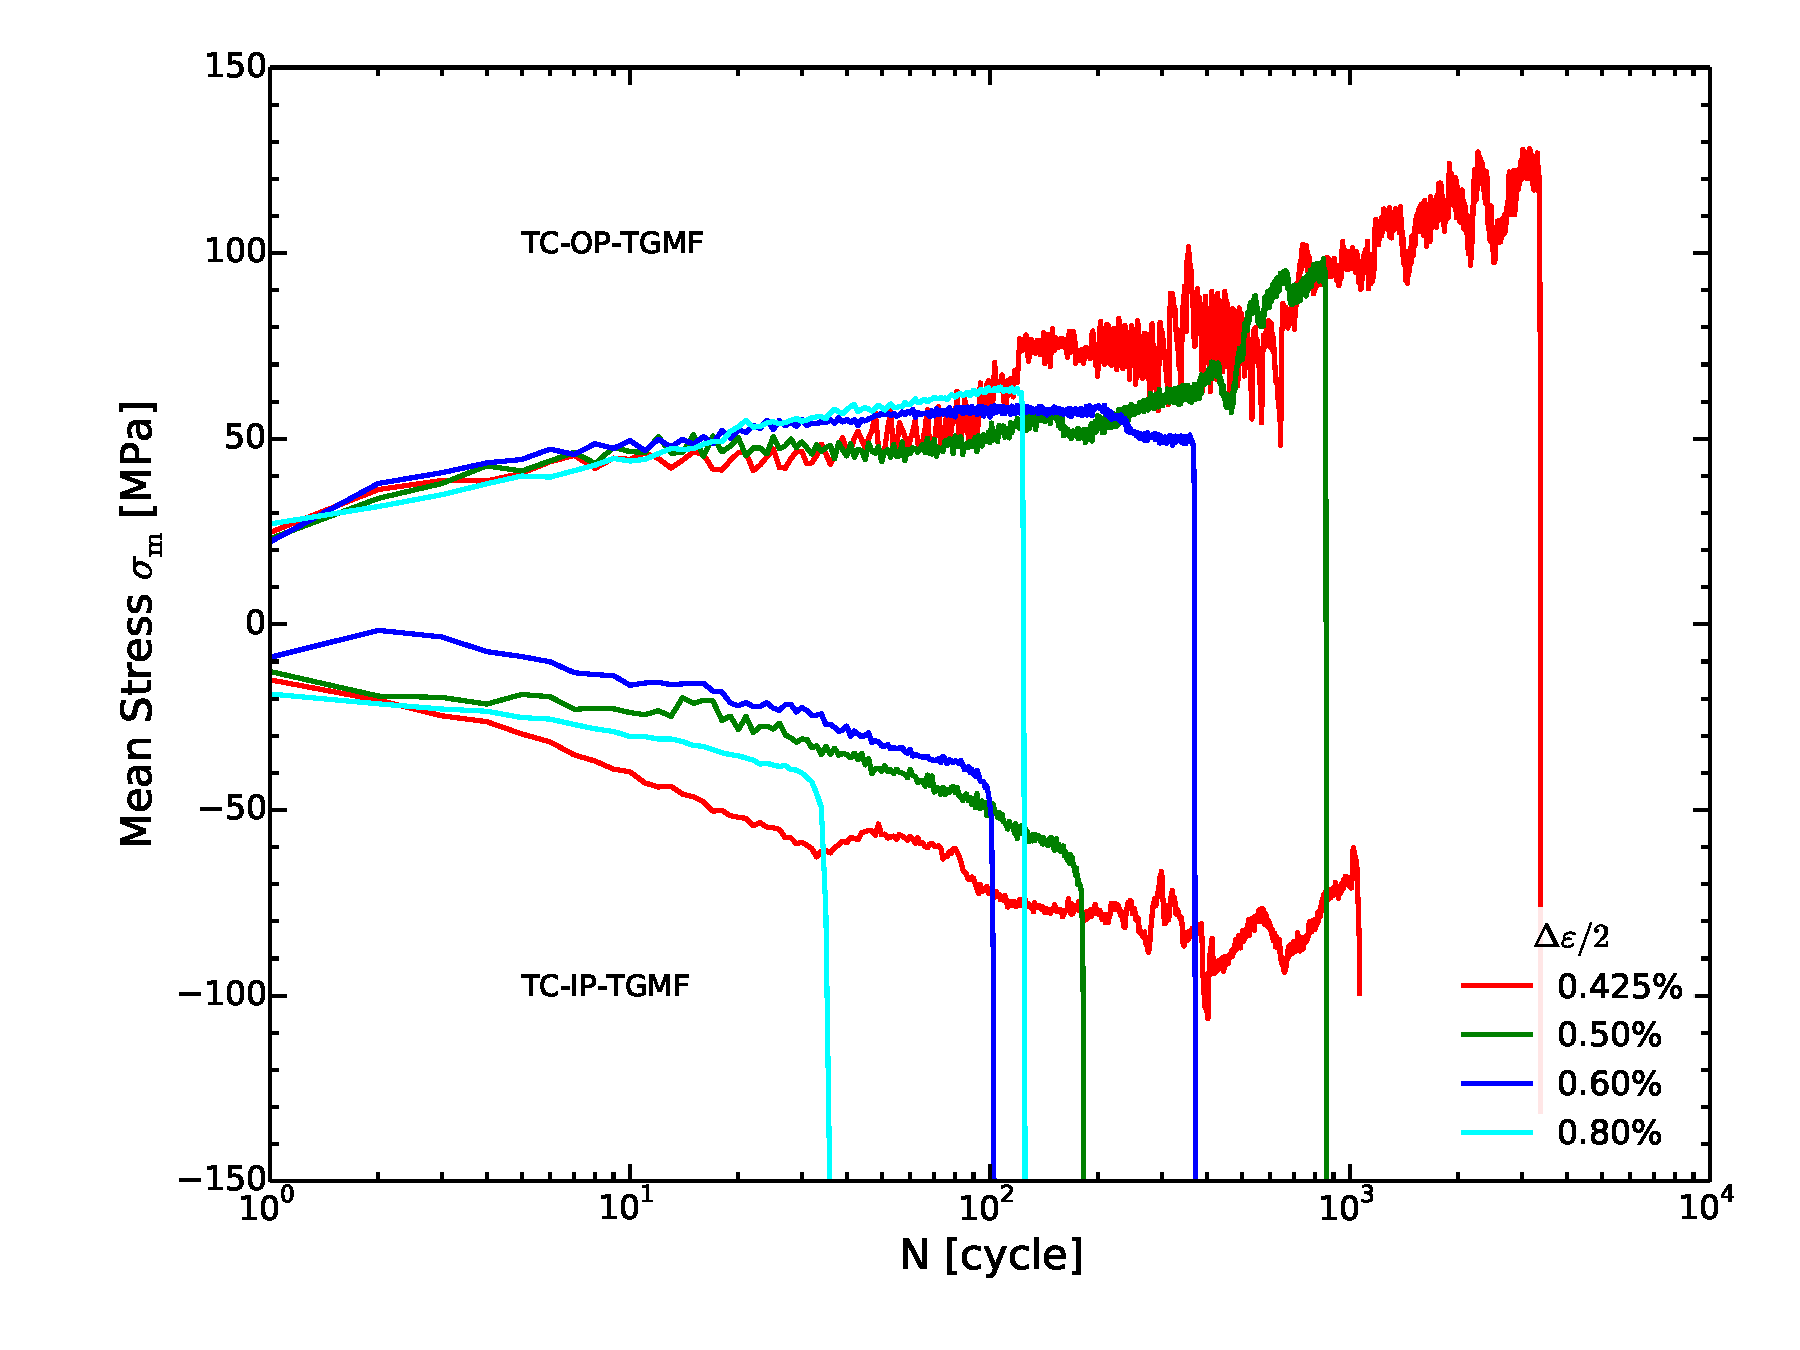
\includegraphics[width=7.5cm]{plot_exp_mean_TCTGMF.pdf}}
  \caption{The evolution of mean stresses under TMF-IP-TGMP and TMF-OP-TGMP loading conditions.}
  \label{Fig:plot_exp_mean_TCTGMF}
\end{figure}

Figures  \ref{Fig:plot_exp_TCTGMF}(b) and (d) illustrate the peak, valley and mean values of the stress response in the TGMF-IP and TGMF-OP tests, respectively.
Cyclic softening were observed during in in-phase and out-of-phase thermal gradient mechanical fatigue tests, but the phase difference between the temperature cycle and the load cycle leads to the different cycle softening behavior. In the temperature range of 300$^\circ$C to 650$^\circ$C, the higher is the temperature, the more obvious the cyclic softening of the material becomes. Therefore, under the TGMF-IP loading condition, the cyclic softening of the superalloy in the tensile half cycle is more evident, whereas the TGMF-OP load made the cyclic softening behavior more clear in the compressive half cycle. 

The mean stress cannot be ignored in low cycle fatigue. Especially for nickel-based superalloys with high strength and low toughness, the mean stress is an important factor affecting the fatigue life, as shown in \autoref{Fig:plot_exp_mean_TCTGMF}. The mean stress response curve for the Inconel 718 alloy under the in-phase and reverse phase TGMF test conditions. It can be seen that for TGMF-IP, the mean stress is compressive stress, and the increase of the mechanical strain amplitude has few effects on the mean stress. For TGMF-IP test, the mean stress becomes a compression stress since the lower temperature stress is compressive. When $\Delta \varepsilon=0.8\%$, the mean stress at the half-life cycle is about -30 MPa.  For TGMF-OP test, the mean stress becomes tensile and increases with the mechanical strain amplitude.
When $\Delta \varepsilon=0.8\%$, the mean stress at the half-life cycle is about 50 MPa. The asymmetry of cyclic softening in tension and compression results in variations of the mean stress in the fatigue tests towards the lower temperature loading direction. For different mechanical strain amplitudes, the mean stress evolution rate is similar, and the mean stress value increases with the number of cycles.

The evolution of mean stress in TGMF is that the strength of the alloy changes with temperature. Both in-phase and out-of-phase TGMF tests, the temperature cycles in the interval of 300$^\circ$C to 650$^\circ$C. When the temperature is high, the strength of the alloy is low. On the contrary, when the temperature is low, the strength of the alloy becomes high. It results in the stress asymmetry of the hysteresis loop. The mean stress develops towards to the low-temperature half cycle.
The reason is that with the increase of the mechanical strain amplitude, the plastic deformation of the alloy at the high-temperature half cycle increases, which aggravates the asymmetry of tensile and compressive stress.
Additionally, it can be observed that the absolute value of the mean stresses increases gradually with cycling under TGMF loading conditions, which can be considered as a result of the more intense softening of the superalloy Inconel 718 during the high-temperature half cycle. In the isothermal fatigue test, the mean stress value is generally small, so the mean stress has  negligible variations on the isothermal fatigue test.

\begin{figure}[!ht]
\centering{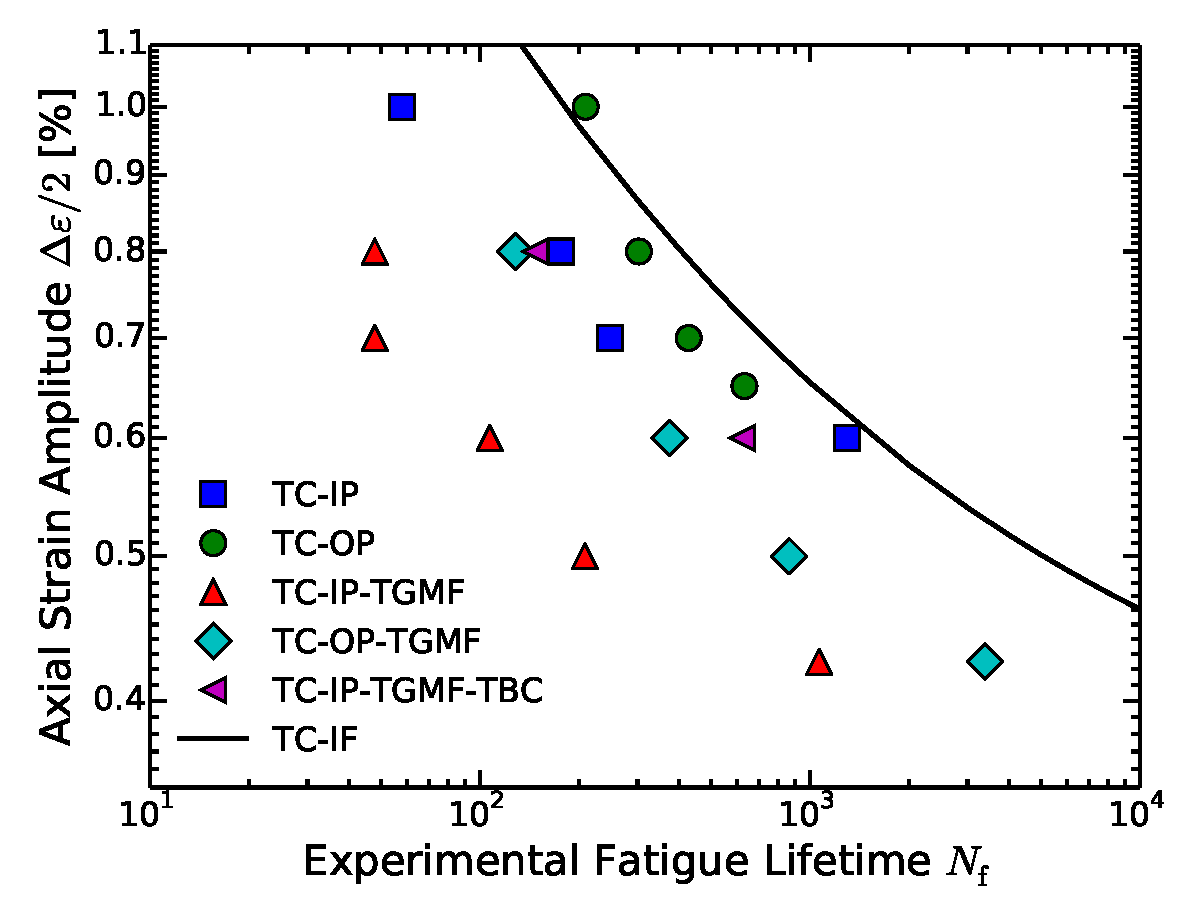
\includegraphics[width=7.5cm]{plot_exp_fatigue_life_TGMF.pdf}}
\caption{Comparison of the fatigue lives under IF, TMF and TGMF loading conditions.}
\label{Fig:plot_exp_fatigue_life_TGMF}
\end{figure}

For fatigue tests under mechanical strain control, the fatigue life can generally be expressed as a function of mechanical strain amplitude.
\autoref{Fig:plot_exp_fatigue_life_TGMF} shows the comparison of the fatigue lifetimes of TMF and TGMF tests under in-phase and out-of-phase loading conditions, respectively. The scattering of the experimental data is dramatic, although the isothermal fatigue life (IF) was obtained from the material for the higher temperature 650\degreeC. All the TMF and TGMF results show lower fatigue lives than the IF. The assessment based on the isothermal fatigue at the higher temperature is not conservative for the Inconel 718.
The TGMF-IP life is much smaller than the TMF-IP life, as shown in \autoref{Fig:plot_exp_fatigue_life_TMF_TGMF_TC}(a) and the TGMF-OP life is smaller than the TMF-OP life, as shown in \autoref{Fig:plot_exp_fatigue_life_TMF_TGMF_TC}(b). However, the difference is substantial. In the figures
the temperature cycles of the TMF and TGMF tests are the same, the only difference between the TMF and TGMF tests is the temperature gradient in the specimen.
Therefore, the temperature gradient is considered to have a significant effect on the fatigue life under the thermo-mechanical loading condition.
Comparing \autoref{Fig:plot_exp_fatigue_life_TMF_TGMF_TC}(a) with \autoref{Fig:plot_exp_fatigue_life_TMF_TGMF_TC}(b), the reduction of TGMF-IP life due to the temperature gradient is more evident than the reduction of TGMF-OP life.

\begin{figure}[!ht]
  \centering
  \begin{overpic}[width=7.5cm]{plot_exp_fatigue_life_IP.pdf}
    \put(84,65){\fcolorbox{white}{white}{(a)}}
  \end{overpic}
  \begin{overpic}[width=7.5cm]{plot_exp_fatigue_life_OP.pdf}
    \put(84,65){\fcolorbox{white}{white}{(b)}}
  \end{overpic}
  \caption{Comparison of fatigue lives of TMF and TGMF: (a) IP, (b) OP.}
  \label{Fig:plot_exp_fatigue_life_TMF_TGMF_TC}
\end{figure}

\section{FEM analysis of thermal gradients}

\subsection{Internal cooling in tabular specimens}

The internal surface of the specimen was cooled with  compressed air, as mentioned before.
Because of the small internal diameter of 6.5 mm in the specimen, it is difficult to measure the temperature of the  specimen surface during tests. 
A variety of measurement options were tried to measure the  surface temperature.
It was found that the internal cooling air has a significant effect on the thermocouple temperature of the inner surface of the specimen.
The thermocouple measurement is not the temperature of the inner surface, but the average temperature of the wall and the cooling air flow.
Therefore, the calibrated finite element computation  becomes an alternative way to obtain the temperature distribution of the specimen inner surface.

\subsection{FE-model}

The geometry of the TGMF specimen is shown in \autoref{Fig:IN718_Axial_Specimen_TGMF}, because of the symmetry of the geometry and the external environment, only the gauge section of the specimen is discretized using axisymmetric  elements. The gauge length is 12 mm, and the center cross-section of the specimen is taken as the symmetric plane for the FEM model. 
The outer surface of the specimen is defined as a temperature boundary condition. The temperature distribution of the outer surface was measured during the test. The inner surface of the specimen is considered as an enforced convection boundary. The convective heat transfer coefficient can be calculated by an empirical formula for turbulent flow in tubes. The density, the temperature and the volume flow of the cooling air need to be measured. The specimen is symmetric about its central cross-section. Therefore, only a half of the specimen is modeled, and the symmetry boundary condition is applied.
The upper surface of the model is considered as a thermal conduction boundary. For radiation calculations, the emissivity of the surface of the specimen is defined as 0.75.

\iffalse
\begin{figure}[!ht]
  \centering{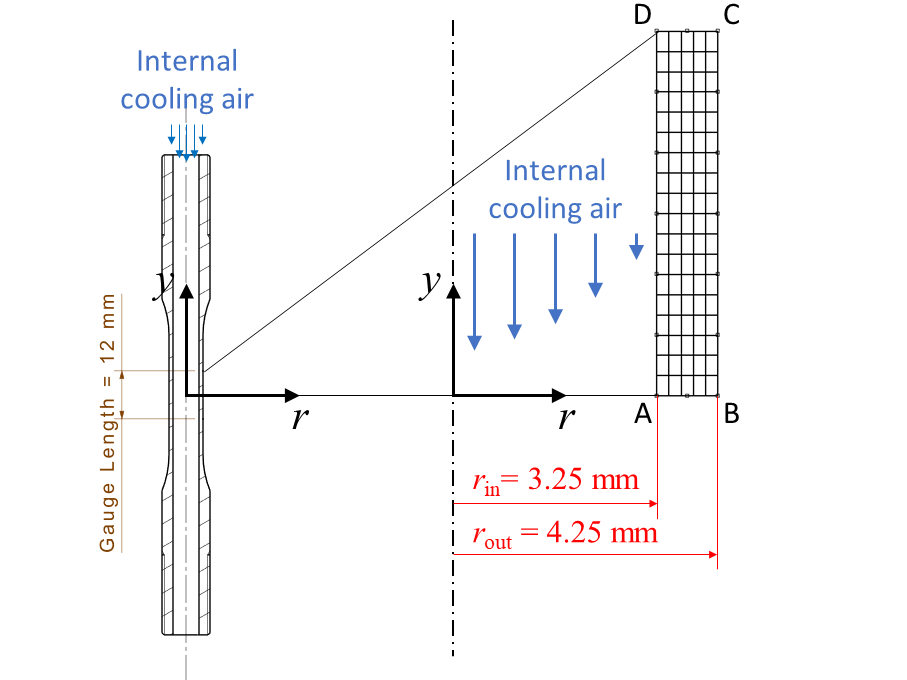
\includegraphics[width=9cm]{FE_model.png}}
  \caption{Schematic diagram of the finite element model.}
  \label{Fig:FE_model}
\end{figure}
\fi

\subsection{Enforced convection in turbulent pipe flow}
The inner surface of the hollow specimen can be considered as a pipe.
%空心试件可以简化为圆管.
According to the formula of convection in turbulent pipe flow, the convective heat transfer coefficient of the inner surface of the specimen can be calculated.
%根据圆管内部的强制对流换热公式,我们计算试件内表面的对流换热系数。

Nusselt number (Nu) is a dimensionless number, defined as the ratio of convective to conductive heat transfer across (normal to) the boundary.
The Nusselt number is given as \marked{(Literature?)}
\begin{equation}
{\rm{N}}{{\rm{u}}_L} = \frac{{hL}}{k},
\end{equation}
where $h$ is the convective heat transfer coefficient of the fluid, $L$ is the characteristic length, $k$ is the thermal conductivity of the fluid.

Gnielinski's correlation for turbulent flow in tubes \marked{(Literature?)} is given as
\begin{equation}
{\rm{N}}{{\rm{u}}_D} = \frac{{\left( {f/8} \right)\left( {{\rm{R}}{{\rm{e}}_D} - 1000} \right){\rm{Pr}}}}{{1 + 12.7{{(f/8)}^{1/2}}\left( {{\rm{P}}{{\rm{r}}^{2/3}} - 1} \right)}},
\end{equation}
where $f$ is the Darcy friction factor that can either be obtained from the Moody chart or for smooth tubes from correlation developed by Petukhov \marked{(Literature?)}
\begin{equation}
f = {\left( {0.79\ln \left( {{\rm{R}}{{\rm{e}}_D}} \right) - 1.64} \right)^{ - 2}},
\end{equation}
with
\begin{equation}
0.5 \le {\rm{Pr}} \le 2000,
\end{equation}
\begin{equation}
3000 \le {\rm{R}}{{\rm{e}}_D} \le 5 \times {10^6},
\end{equation}

The Prandtl number (Pr) is a dimensionless number, defined as the ratio of momentum diffusivity to thermal diffusivity, defined as
\begin{equation}
{\rm{Pr}} = \frac{{{c_p}\mu }}{k},
\end{equation}
where
$c_{p}$ is specific heat, $\mu$ is dynamic viscosity and $k$ is thermal conductivity. For air $c_{p}=903.3 {\rm{J/(kg}} \cdot {\rm{K}})$ and $k=0.0258$ ${\rm{W/(m}} \cdot {\rm{K}})$ at 288.15 ${\rm{K}}$.

The Reynolds number (Re) is a dimensionless number, defined as the ratio of inertial forces to viscous forces within a fluid.
The Reynolds number is given as:
\begin{equation}
{\rm{Re}} = \frac{{\rho uL}}{\mu },
\end{equation}
where
$\rho$ is the density of the fluid, $u$ is the velocity of the fluid with respect to the object, $\mu$ is the dynamic viscosity of the fluid, and $L$ is a characteristic dimension.
It is noted that the dynamic viscosity $\mu$ of an ideal gas is a function of the temperature. The Sutherland's formula can be derived as follows
\begin{equation}
\mu  = {\mu _0}\frac{{{T_0} + C}}{{T + C}}{\left( {\frac{T}{{{T_0}}}} \right)^{\frac{3}{2}}},
\end{equation}
where 
$\mu_0$ is the reference viscosity at reference temperature $T_0$,
$C$ is Sutherland's constant depending on the gaseous material. For air at $T_0=291.15 $K the the reference viscosity $\mu_0=1.827\times 10^{-5} \rm{Pa\cdot s}$ and Sutherland's constant $C=120$K.

The density of dry air $\rho$ can be calculated using the ideal gas law, expressed as a function of temperature and pressure, as 
\begin{equation}
\rho  = \frac{p}{{RT}},
\label{Equ:AirDensity}
\end{equation}
where
$p$ is absolute pressure,
$T$ is absolute temperature,
$R$ is specific gas constant and equals 287.058${\rm{J/(kg}} \cdot {\rm{K}})$.

According to the measurement results of the sensors, the average pressure and temperature of the cooling air are 6.5 bar and 288.15 K, respectively.

\begin{table}[!ht]
\centering
  \begin{threeparttable}
  \centering
  \caption{Heat convection coefficients of the inner surface of the specimen.}
    \begin{tabular}{p{2cm}p{2cm}p{2cm}}
    \toprule
    Quantity   & Unit & Value  \\
    \midrule
    $T$   & ${\rm{K}}$ & 288.15  \\
    $p$   & ${\rm{bar}}$ & 6.5   \\
    $\rho$& ${\rm{kg/}}{{\rm{m}}^{\rm{3}}}$ & 7.724 \\
    $\mu$ & -     & 1.81E-05 \\
    ${\dot V}$ & ${\rm{l/min}}$ & 40  \\
%    $u$ \tnote{*3} & ${\rm{m/}}{{\rm{s}}^2}$ & 20.09  \\
    ${\rm{Re}}$ & -     & 55624  \\
    ${\rm{Pr}}$ & -     & 0.63  \\
    $f $ & -     & 0.0205  \\
    ${\rm{N}}{{\rm{u}}_D} $ & -     & 106.50  \\
    $h $ & ${\rm{W/(}}{{\rm{m}}^{\rm{2}}} \cdot {\rm{K)}}$ & 423.10  \\
    \bottomrule
    \end{tabular}%
    \end{threeparttable}
  \label{tab:addlabel}%
\end{table}%
\renewcommand\arraystretch{1}


\begin{figure*}[!h]
  \centering
  \begin{overpic}[width=7.5cm]{plot_cmp_half_life_cycle_TCIPTGMF.pdf}
    \put(84,65){\fcolorbox{white}{white}{(a)}}
  \end{overpic}
  \begin{overpic}[width=7.5cm]{plot_cmp_pv_TCIPTGMF.pdf}
    \put(84,13){\fcolorbox{white}{white}{(b)}}
  \end{overpic}

  \begin{overpic}[width=7.5cm]{plot_cmp_half_life_cycle_TCOPTGMF.pdf}
    \put(84,13){\fcolorbox{white}{white}{(c)}}
  \end{overpic}
  \begin{overpic}[width=7.5cm]{plot_cmp_pv_TCOPTGMF.pdf}
    \put(84,13){\fcolorbox{white}{white}{(d)}}
  \end{overpic}
  \caption{Experimental and computational results under the thermal gradient mechanical loading conditions with varying temperature between 300$^\circ$C and 650$^\circ$C. The vertical axis the nominal normal stress. (a) The hysteresis loops of TGMF-IP tests. (b) Peak, valley and mean stress values of TGMF-IP tests. (c) The hysteresis loops of TGMF-OP tests. (d) Peak, valley and mean stress values of TGMF-OP tests.}
  \label{Fig:plot_exp_fatigue_life_TMF_TGMF}
\end{figure*}


\begin{figure*}
  \centering{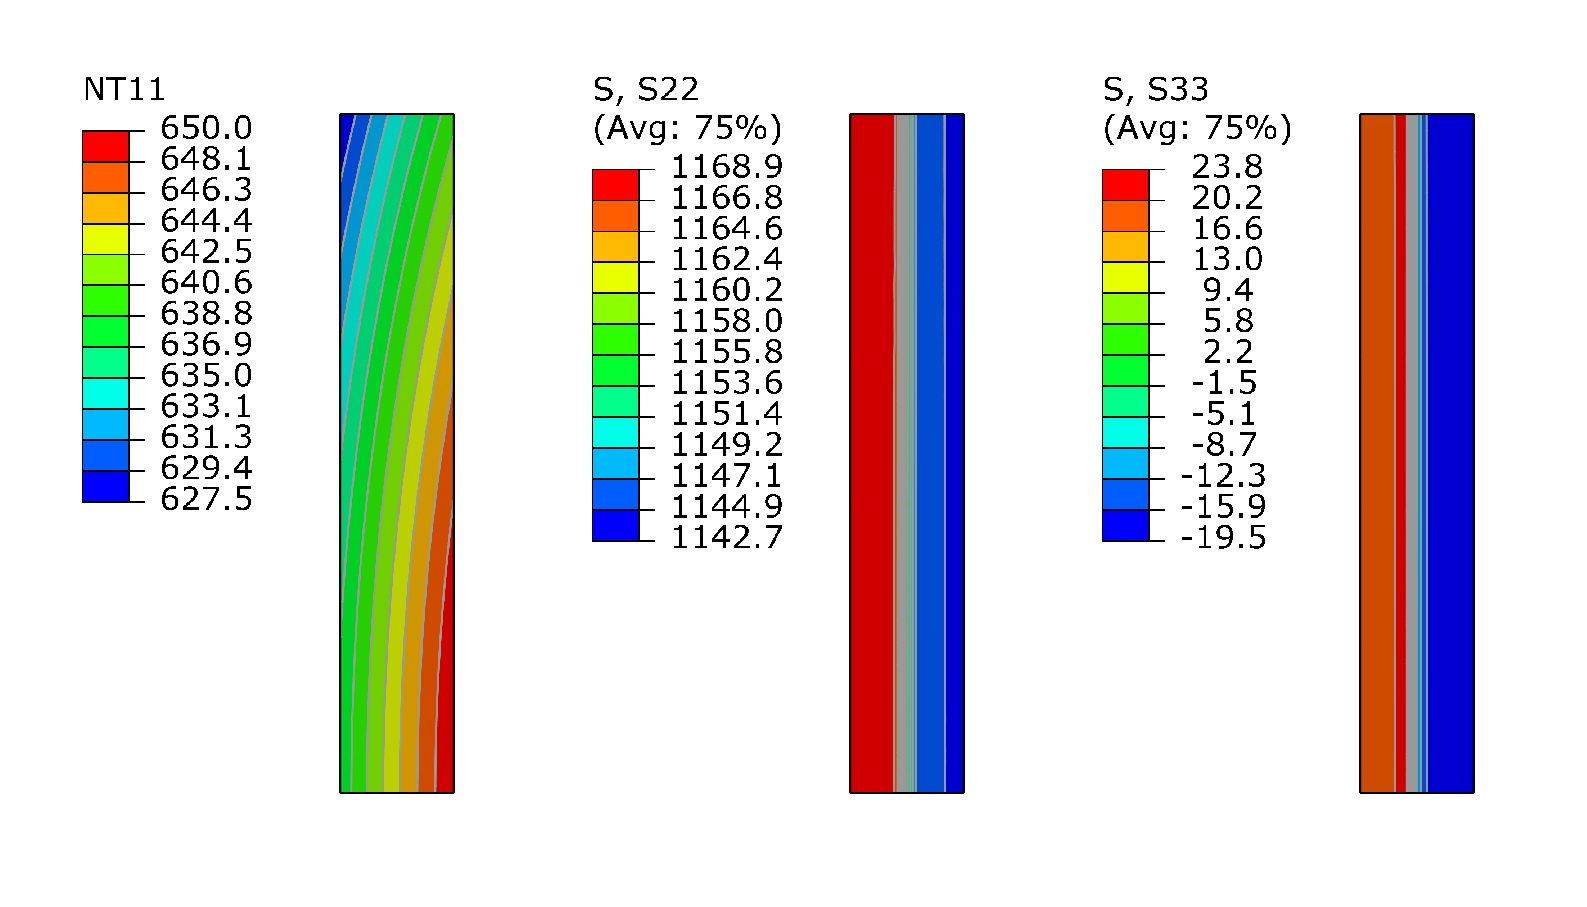
\includegraphics[width=13cm]{FEM_result.jpg}}
  \caption{Computational distributions of axial temperature and the temperature-gradient-induced stress components at maximum temperature (650$^{\circ}$C) during the TGMF-IP test with the mechanical strain amplitude of 0.8\%.  (a) Temperature NT11 in ℃; (b) Axial stress S22 in MPa; (c) Hoop stress S33 in MPa).}
  \label{Fig:FEM_result}
\end{figure*}

\subsection{Computational results}
% 图\autoref{Fig:plot_temperature_along_gauge_length}为试件内、外表面温度和轴向应力在标距段内沿轴向的分布,横坐标为距离试件中心截面的距离,在TGMF-IP循环过程中,图中所示的温度与应变为温度最高点(650$^{\circ}$C)时的值。
% 此时,试件外表面与内表面的温差为12.5$^{\circ}$C,

The constitutive behavior of the superalloy Inconel 718 under multiaxial thermo-mechanical loading was studied and a constitutive equation for TMF was introduced and implemented into the commercial FEM software  ABAQUS \cite{SUN2019228, SUN201989}, which are used in the present finite element computations. Figs. \ref{Fig:plot_exp_fatigue_life_TMF_TGMF} (a) and (c) show that the experimental and computational stress-strain responses of the TGMF-IP and TGMF-OP tests, respectively. The vertical coordinates are the nominal stress, and the horizontal coordinates are the nominal mechanical strain in the center cross-section of the specimen. Because of the thermal gradient, the cyclic plastic evolutions were asymmetric in the gauge section of the specimen in the TGMF tests. In the figures, additional tensile strains were observed from the computational results of the TGMF-IP tests, and additional compressive strains were found from the computational results of the TGMF-OP tests. Figs. \ref{Fig:plot_exp_fatigue_life_TMF_TGMF} (b) and (d) show the experimental and computational peak, valley and mean nominal stresses of the TGMF-IP and TGMF-OP tests, respectively. The comparison of the experimental and computational results reveals that the proposed constitutive model can describe elastic-plastic mechanical behavior under the thermal gradient mechanical loading conditions. Therefore, the computed local stress-strain responses are used for the life assessment of TGMF. Effects of the TGMF seem not large to the constitutive behavior of the material.

\begin{figure}[!ht]
  \centering
    \begin{overpic}[width=7.5cm]{plot_temperature_along_gauge_length.pdf}
      \put(75,65){\fcolorbox{white}{white}{(a)}}
    \end{overpic}
    \begin{overpic}[width=7.5cm]{plot_temperature_along_radial_direction.pdf}
      \put(75,65){\fcolorbox{white}{white}{(b)}}
    \end{overpic}
  \caption{Computational distributions of the temperature and normal stresses at the maximum temperature (650$^\circ$C) during the TGMF-IP test with the mechanical strain amplitude of 0.8\%. (a) The axial distribution; (b) the radial distribution.}
  \label{Fig:plot_temperature_stress}
\end{figure}

Under TGMF-IP loading condition, the mechanical load and temperature simultaneously reach their respective maximum or minimum values. \autoref{Fig:FEM_result} shows the computational results of TGMF-IP test with the mechanical strain amplitude of 0.8\%. The maximum temperature occurs at the symmetric position of the outer surface of the specimen.
\autoref{Fig:plot_temperature_stress}(a) illustrates the temperature and axial stress distribution of the internal and external surface along the axial direction when the temperature reached its maximum value during the TGMF-IP cycle.
The abscissa axis is the distance from the center section of the test specimen ($y$-axis). The temperature gradients induce an axial stress difference of ca. 25 MPa between the inner and outer surface of the specimen.
The temperature and axial stress distribution of the internal and external surface along the radial direction are displayed in \autoref{Fig:plot_temperature_stress}(b), when the temperature reached its maximum value during the TGMF-IP cycle.
The abscissa axis is the distance from the center axis to the outer surface of the test specimen.
The temperature gradients induce a radial stress deviation of ca. 50 MPa between the inner and outer surface of the specimen.  

Obviously, the computational results do not contain influence of the gravitation in heat convection. Due to thermal expansion in air both ends of the specimen are cooled differently, which is not included in the present analysis. However, the present computations give a reliable estimate of the temperature distribution during the TGMF tests.


\begin{figure}[ht]
  \centering
    \begin{overpic}[width=7.5cm]{7206-1.jpg}
      \put(0,65){\fcolorbox{white}{white}{(a)}}
      \put(70,40){\color{white}\thicklines\vector(3,-1){20}}
    \end{overpic}
    \begin{overpic}[width=7.5cm]{7207-1.jpg}
      \put(0,65){\fcolorbox{white}{white}{(b)}}
      \put(60,40){\color{white}\thicklines\vector(1,-1){13}}
    \end{overpic}
  \caption{Locations of crack initiation from the TGMF tests: (a) TGMF-IP 0.65\%, (b) TGMF-OP 0.65\%. Arrows denote the crack initiation locations.}
  \label{Fig:crack_initiation_TGMF}
\end{figure}


\section{Fatigue life assessment of TGMF}

\subsection{Fractography}

Analysis of fractography provides the locations of the crack initiation, the crack propagation and the direction of the fatigue striation.
Typical fractographs in the region of crack initiation are shown in \autoref{Fig:crack_initiation_TGMF}, and the arrows show the locations of the crack initiation. For both TGMF-IP and TGMF-OP loadings, crack initiation and subsequent failure have been identified as being initiated at the outer surface of the specimen.

Figure \ref{Fig:fatigue_striations_TGMF} shows the fractography of stable crack propagation. For the TGMF tests, the SEM investigations reveal that the dominant failure mechanism is changing with the phase angle of the thermal loading and mechanical loading, $\theta_{T-\varepsilon}$.
In \autoref{Fig:fatigue_striations_TGMF}(a) and (b), the fracture surfaces under TGMF-IP loading displays evident grain boundaries and slight fatigue striations. Consequently, it can be concluded that a mixture of transgranular and intergranular fracture mode is present in the TGMF-IP test, and the intergranular fracture plays a dominant role.
Well-developed fatigue striations are observed in \autoref{Fig:fatigue_striations_TGMF}(c) and (d), which reveal transgranular crack growth is predominant during out-of-phase thermo-mechanical tests.

\begin{figure*}[!ht]
  \centering{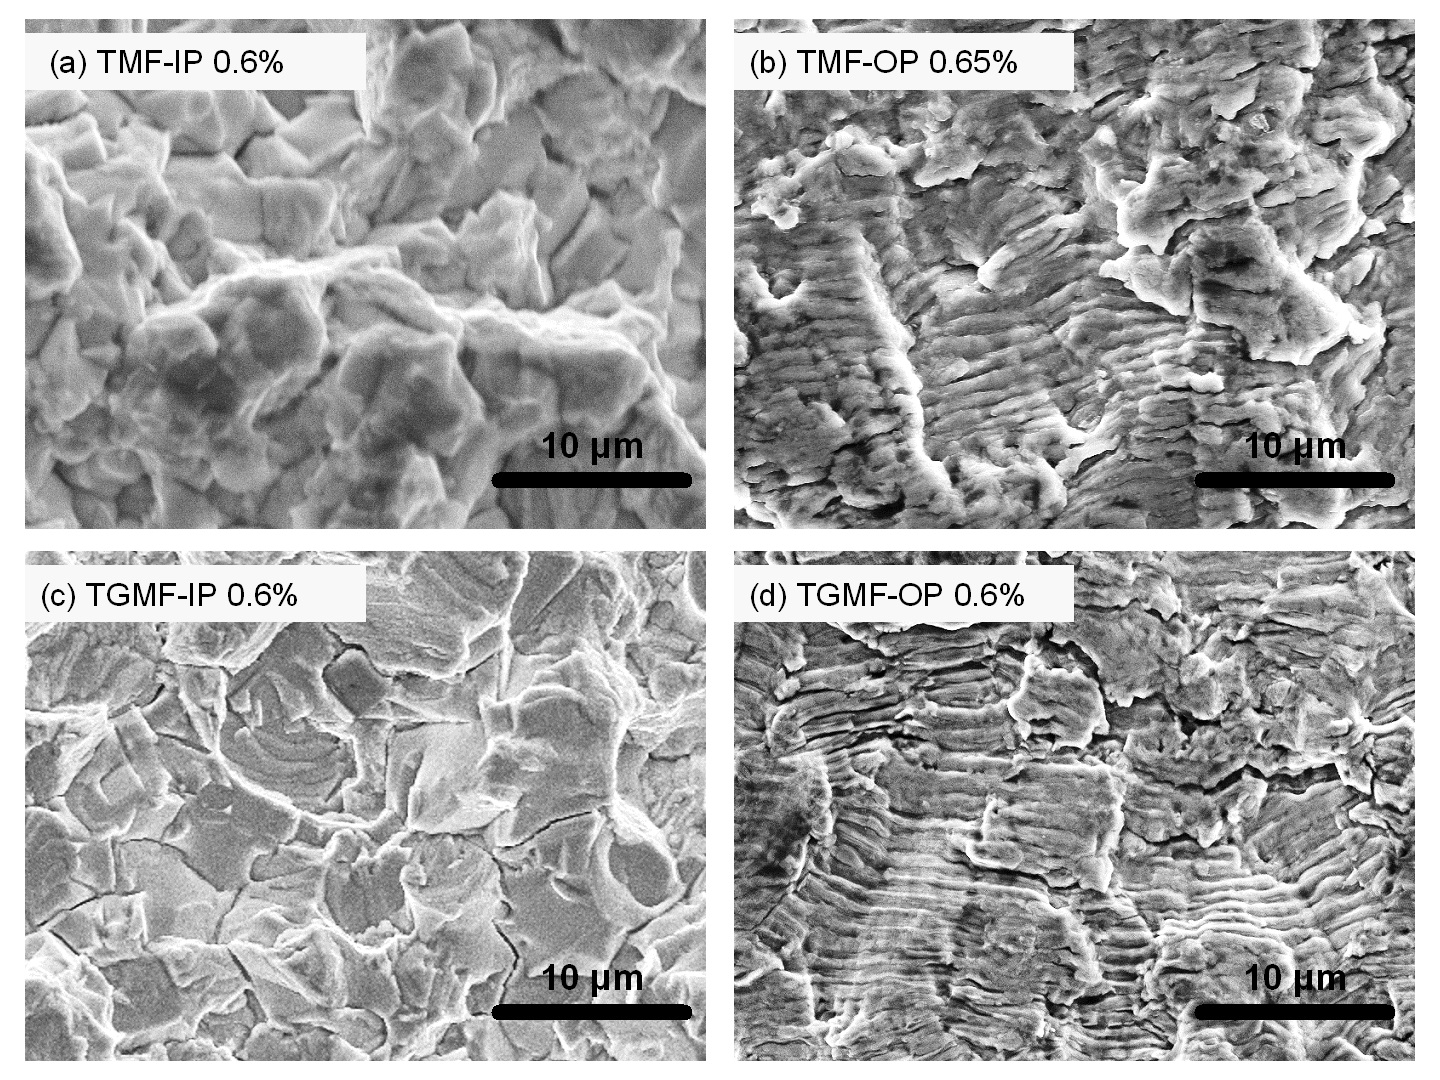
\includegraphics[width=14cm]{Fractography.jpg}}
  \caption{Fractographs of fracture surfaces from the area of stable crack propagation.}
  \label{Fig:fatigue_striations_TGMF}
\end{figure*}

The present fractographic analysis confirms that the TGMF failure mechanisms are similar of the high temperature fatigue. All specimens show fatigue crack nucleation occurs in the specimen surfaces, which implies that the TGMF could be assessed by the conventional or TMF fatigue failure models. In the present section, several known fatigue models are selected to evaluate the fatigue life of the nickel-based superalloy under both TMF and TMGF loading conditions. Combined with the critical plane concept the models are well developed and verified for isothermal fatigue.


\subsection{Brown-Miller Model}
{Based on the critical plane concepts \cite{Brown2006}, Wang and Brown \cite{Wang1993} proposed a  fatigue model in the form of the equivalent shear strain amplitude}, as
\begin{equation}
\frac{{\Delta \hat \gamma }}{2} = \frac{{\Delta {\gamma _{\max}}}}{2} + S\Delta {\varepsilon _{\rm n}},
\label{Equ:ShearStrainBM}
\end{equation}
where ${{\Delta \hat \gamma }}/{2}$ is the equivalent shear strain range \cite{Wang1993}. $\Delta {\varepsilon _{\rm n}}$ represents the normal strain acting on the plane with the maximum shear strain range $\Delta {\gamma _{\max}}$. The material dependent parameter $S$ represents the influence of the normal strain on the crack propagation.
The fatigue endurance is determined from 
\begin{equation}
\frac{{\Delta \hat \gamma }}{2} = A\frac{{{{\sigma '}_{\rm f}}}}{E}{\left( {2{N_{\rm f}}} \right)^b} + B{{\varepsilon '}_{\rm f}}{\left( {2{N_{\rm f}}} \right)^c}
\end{equation}
with
\[A = 1 + {\nu _{\rm e}} + \left( {1 - {\nu _{\rm e}}} \right)S\]
and
\[B = 1 + {\nu _{\rm p}} + \left( {1 - {\nu _{\rm p}}} \right)S.\]


\subsection{Fatemi-Socie model}
Fatemi and Socie \cite{Fatemi1988} proposed that the normal strain term in Eq. (\ref{Equ:ShearStrainBM}) should be replaced by the normal stress.
The equivalent shear strain amplitude is defined as
\begin{equation}
\frac{{\Delta \hat \gamma }}{2} = \frac{{\Delta {\gamma _{\max }}}}{2}\left( {1 + k\frac{{{\sigma _{\rm n,\max}}}}{{{\sigma _{\rm y}}}}} \right),
\end{equation}
where
$\sigma _{\rm n,\max}$ is the maximum normal stress on the critical plane suffering from the maximum shear strain range $\Delta {\gamma _{\max}}$, and $k$ is a material parameter. The sensitivity of the material to the normal stress is reflected in the ratio $k/\sigma _{\rm y}$.
The fatigue life model oriented to the shear-based damage is illustrated as
\begin{equation}
\frac{{\Delta \hat \gamma }}{2} = \frac{{{{\tau '}_{\rm f}}}}{G}{\left( {2{N_{\rm f}}} \right)^{{b_0}}} + {{\gamma '}_{\rm f}}{\left( {2{N_{\rm f}}} \right)^{{c_0}}}.
\end{equation}
Furthermore, McClaflin and Fatemi \cite{McClaflin2004} proposed that the sensitivity parameter $k$ varies with fatigue life and can be related to the tension and torsion property, that is,
\begin{equation}
k =  \frac{{k_0 {\sigma _{\rm y}}}}{{{{\sigma '}_{\rm f}}{{\left( {2{N_{\rm f}}} \right)}^b}}}
\end{equation}
with
\[
k_0 =  {\frac{{\frac{{{{\tau '}_{\rm f}}}}{G}{{\left( {2{N_{\rm f}}} \right)}^{{b_0}}} + {{\gamma '}_{\rm f}}{{\left( {2{N_{\rm f}}} \right)}^{{c_0}}}}}{{\left( {1 + {\nu _{\rm e}}} \right)\frac{{{{\sigma '}_{\rm f}}}}{E}{{\left( {2{N_{\rm f}}} \right)}^b} + \left( {1 + {\nu _{\rm p}}} \right){{\varepsilon '}_{\rm f}}{{\left( {2{N_{\rm f}}} \right)}^c}}} - 1} .
\]

%where the equivalent shear strain on the critical plane was based on a combination of the maximum shear strain amplitude $\Delta \gamma$ and maximum normal stress $\sigma _{\rm n, \max}$ during the cycle. The shear strain was used as the variable decisive for the rain-flow decomposition.
%The criterion used to be based on the MSSR maximization.

\subsection{Smith-Watson-Topper model}
The SWT model \cite{smith1970stress} can be extended to multiaxial fatigue assessment based on the principal strain range and the maximum stress on the plane of the principal strain range, that is,
\[
{\sigma _{\rm n, \max}}\frac{{\Delta \varepsilon }}{2} = \frac{{{{\sigma '}_{\rm f}}^2}}{E}{\left( {2{N_{\rm f}}} \right)^{2b}} + {\sigma '_{\rm f}}{\varepsilon '_{\rm f}}{\left( {2{N_{\rm f}}} \right)^{b + c}}.
\]

\subsection{Liu's virtual strain energy models}
The virtual tensile strain energy based model suggested by Liu \cite{Liu1993} can be written as
\begin{eqnarray*}
{\left( {\Delta {\sigma _{\rm n}}\Delta {\varepsilon _{\rm n}}} \right)_{\max }} + \left( {\Delta \tau \Delta \gamma } \right) &=& \frac{{4{{\sigma '}_{\rm f}}^2}}{E}{\left( {2{N_{\rm f}}} \right)^{2b}}
\\
& & + 4{{\sigma '}_{\rm f}}{{\varepsilon '}_{\rm f}}{\left( {2{N_{\rm f}}} \right)^{b + c}}.
\end{eqnarray*}
Above the critical plane is defined from maximizing the virtual tensile strain energy ${\Delta {\sigma _{\rm n}}\Delta {\varepsilon _{\rm n}}}$, termed as Liu I model. Note the model parameters in the present model differ from the others. The corresponding virtual shear strain energy model (Liu II model) is expressed as
\begin{eqnarray*}
\left( {\Delta {\sigma _{\rm n}}\Delta {\varepsilon _{\rm n}}} \right) + {\left( {\Delta \tau \Delta \gamma } \right)_{\max }} &=& \frac{{4{{\tau '}_{\rm f}}^2}}{G}{\left( {2{N_{\rm f}}} \right)^{2b_0 }}
\\
&& + 4{{\tau '}_{\rm f}}{{\gamma '}_{\rm f}}{\left( {2{N_{\rm f}}} \right)^{b_0  + c_0 }}.
\end{eqnarray*}
The critical plane is calculated from the virtual shear strain energy \cite{Liu1993}.

\subsection{Chu-Conle-Bonnen model}
An additional energy-based fatigue model suggested by Chu et al. \cite{Chu1993} is expressed as
\begin{eqnarray*}
{\left( {{\tau _{\rm n}}\frac{{\Delta \gamma }}{2} + {\sigma _{\rm n }}\frac{{\Delta \varepsilon }}{2}} \right)_{\max }} &=& 1.02\frac{{{{\sigma '}_{\rm f}}^2}}{E}{\left( {2{N_{\rm f}}} \right)^{2b}} \\
&& + 1.04{{\sigma '}_{\rm f}}{{\varepsilon '}_{\rm f}}{\left( {2{N_{\rm f}}} \right)^{b + c}}.
\end{eqnarray*}
Note the difference in the strain energy in comparing with the Liu's models. The critical plane should provide the maximum strain energy in the whole loading range and in all directions.


\subsection{TMF Model suggested by Sun and Yuan  \cite{SUN2019228}}
Based on the Liu's virtual tension strain energy model, Sun and Yuan \cite{SUN2019228} introduced a fatigue model for the multi-axial TMF life prediction, as
\begin{equation}
\begin{aligned}
\left[ {A{{\left( {\Delta {\sigma _{\rm n}}\Delta {\varepsilon _{\rm n}}} \right)}_{\max }} + B\left( {\Delta \tau \Delta \gamma } \right)} \right]\left( {\frac{2}{{1 - {R_\sigma }}}} \right)\\
= \frac{{4{{\sigma '}_{\rm f}}^2}}{E}{\left( {2{N_{\rm f}}} \right)^{2b}} + 4{{\sigma '}_{\rm f}}{{\varepsilon '}_{\rm f}}{\left( {2{N_{\rm f}}} \right)^{b + c}}
\end{aligned}
\label{Equ:TMF_model}
\end{equation}
with $A$ defined as
\begin{equation}
A = {\left[ {1 + C\int_{{t_0}}^{{t_0} + {t_{cyc}}} {\eta \left( t \right)\exp \left( {\frac{{ - Q\left( t \right)}}{{RT\left( t \right)}}} \right){\rm{d}}t} } \right]^k},
\label{Equ:A}
\end{equation}
where $\eta \left( t \right)$ is stress triaxiality, $R$ is the ideal gas constant ($8.31\times10^{-3}$ kJ/mol$\cdot$K), the time integral is from the start time $t_0$ of the cycle to the end time $t_0 + t_{cyc}$, $t_{cyc}$ is the period of the tests, $C$ and $k$ are material constants.
In Eq. (\ref{Equ:A}), $Q$ is defined as \cite{Warren2006,Warren2008}
\begin{equation}
Q\left( t \right) = {Q_0} - \upsilon _0^*{\sigma _{\rm n}}\left( t \right)\left( {1 - \frac{{{\sigma _{\rm n}}\left( t \right)}}{{2{\sigma _{\rm ult}}}}} \right),
\label{Equ:creep_activation_energy}
\end{equation}
where $Q_0$ is the the intrinsic activation energy, $\upsilon _0^*$ represents the intrinsic activation volume, $\sigma_{\rm ult}$ is the ultimate stress at the maximum temperature and $\sigma_{\rm n}(t)$ is the normal stress of the critical plane.
As given in \cite{Warren2008}, the activation energy $Q_0$ is set to 240 kJ/mol and the intrinsic activation volume $\upsilon _0^*$ is $3.51\times10^{-4}$ $\rm{m}^{3}/\rm{mol}$. The ultimate strength $\sigma_{\rm ult}$ of Inconel 718 at 650$^\circ$C was measured as $1305$ MPa in monotonic tensile tests. The coefficients $k$, $B$ and $C$ are determined from minimizing the life prediction mean square error. Finally, $k$ equals 1.2, $B$ is 0.49, and $C$ is set to $1.29\times10^{12}$ s$^{-1}$.

\subsection{Fatigue life prediction based on the known fatigue models}
The Brown-Miller's model, Fatemi-Socie's model, Smith-Watson-Topper's model, Chu-Conle-Bonnen's model, Liu's Energy model and TMF model (Eq. \eqref{Equ:TMF_model}) are tried to evaluate the thermal gradient mechanical fatigue.
\autoref{Fig:life_prediction_TGMF} summarizes the comparison between predicted and experimental fatigue life of the IF, TMF-IP, TMF-OP, TGMF-IP and TGMF-OP tests. 

\begin{figure*}
   \centering
   \begin{overpic}[width=7.0cm]{NF-NP-TGMF-BM.pdf}
     \put(65,20){\fcolorbox{white}{white}{(a) BM}}
   \end{overpic}
   \begin{overpic}[width=7.0cm]{NF-NP-TGMF-FS.pdf}
     \put(70,20){\fcolorbox{white}{white}{(b) FS}}
   \end{overpic}

   \begin{overpic}[width=7.0cm]{NF-NP-TGMF-SWT.pdf}
     \put(70,20){\fcolorbox{white}{white}{(c) SWT}}
   \end{overpic}
   \begin{overpic}[width=7.0cm]{NF-NP-TGMF-Chu.pdf}
     \put(70,20){\fcolorbox{white}{white}{(d) CCB}}
   \end{overpic}

   \begin{overpic}[width=7.0cm]{NF-NP-TGMF-Liu1.pdf}
     \put(70,20){\fcolorbox{white}{white}{(e) Liu I}}
   \end{overpic}
   \begin{overpic}[width=7.0cm]{NF-NP-TGMF-Study.pdf}
     \put(70,20){\fcolorbox{white}{white}{(f) TMF}}
   \end{overpic}
  \caption{Comparison between predicted fatigue life and experimental results of thermomechanical as well as thermal gradient mechanical  fatigue tests. (a) Brown-Miller model; (b) Fatemi-Socie model; (c) Smith-Watson-Topper model; (d) Chu-Conle-Bonnen model; (e) Liu Tension Energy model; (f) TMF model  \cite{SUN2019228}.}
  \label{Fig:life_prediction_TGMF}
\end{figure*}

To give a quantitative assessment of the fatigue models, two statistical parameters are used to evaluate the conformity of the predicted fatigue life, $N_{\rm p}$, and the experimental result, $N_{\rm f}$  \cite{KAROLCZUK201439,WALAT201473,SKIBICKI201718, SUN2019228}. 
The mean scatter of fatigue life is defined as
\begin{equation}\label{Equ:TN}
{T_{\rm N}} = {10^{\bar E}}
\end{equation}
with
\begin{equation}
\bar E = \frac{1}{n}\sum\limits_{i = 1}^n {\log \left( {\frac{{{N_{{\rm f},i}}}}{{{N_{{\rm p},i}}}}} \right)},
\end{equation}
{illustrates the comparison of the mean value of experimental and predicted lives. Above $n$ is the total number of the compared results, and the subscript $i$ indicates the $i$th result. $T_{\rm N} = 1$ denotes zero discrepancy between experimental mean value and model predictions. $T_{\rm N} > 1$ means the predicted fatigue lives are conservative, and $T_{\rm N} < 1$ means the predicted fatigue lives are non-conservative. The statistical parameter $T_{\rm N}$ does not provide any information on the dispersion of fatigue life.}

The evaluation results are summarized in \autoref{Fig:plot_fatigue_life_quantitative_evaluation_tgmf}(a). As mentioned, all known models are not conservative and contain significant deviations in the mean life, besides the TMF and TGMF (To be introduced in the next section). The TMF model gives the best prediction in the mean  life prediction. The present model gives a reasonable mean life prediction with small amount of conservativity.

The second parameter describes scattering of the data and is the  mean square root error of the fatigue life, defined as
\begin{equation}\label{Equ:TRMS}
{T_{\rm RMS}} = {10^{{E_{\rm RMS}}}},
\end{equation}
with
\begin{equation}
{E_{\rm RMS}} = \sqrt {\frac{1}{n}\sum\limits_{i = 1}^n {\left[{{\log }}\left( {\frac{{{N_{{\rm f},i}}}}{{{N_{{\rm p},i}}}}} \right) \right]^2}}.
\end{equation}
{The  mean square root error is applied to measure the differences between fatigue lives from predictions and experiments. $T_{\rm RMS} = 1$ is the minimum and represents agreement between experimental points and predictions. A larger $T_{\rm RMS}$ value represents the more dispersion between the experimental life and prediction.}

A quantitative assessment of fatigue life prediction results is illustrated in \autoref{Fig:plot_fatigue_life_quantitative_evaluation_tgmf}(b). 
The results in the figures illustrate that, besides TGMF model to be introduced in the next section,  the TMF model introduced in \cite{SUN2019228} provides the best result. 

\begin{figure}[!h]
  \centering
  \begin{overpic}[width=7.5cm]{plot_fatigue_life_quantitative_evaluation_tgmf_TN.png}
  \put(84,65){\fcolorbox{white}{white}{(a)}}
  \end{overpic}
  \begin{overpic}[width=7.5cm]{plot_fatigue_life_quantitative_evaluation_tgmf_TRMS.png}
  \put(84,65){\fcolorbox{white}{white}{(b)}}
  \end{overpic}
  \caption{The quantitative evaluation of the TGMF life prediction results: (a) $T_{\rm{N}}$, (b) $T_{\rm{RMS}}$.}
  \label{Fig:plot_fatigue_life_quantitative_evaluation_tgmf}
\end{figure}


\section{Introduction of a new TGMF life model}

The previous section confirms that all known models do not give reasonable conservative predictions  for the thermal gradient mechanical fatigue tests, since effects of the thermal gradients are too strong to be considered in the conventional fatigue models. In fact the thermal stress is induced by the temperature gradient and cannot be represented by the applied mechanical stress, which is the major difference to the TMF. To give a reasonable prediction of the TGMF life, the temperature gradient has to be included in the life model in a suitable way. 

The TMF model  \cite{SUN2019228}  seems to give the best agreement to both TMF and TGMF tests, but not conservative, and will be extended for TGMF in the present work.
Based on the TMF model, a correction term relying on the temperature gradient is to be included on the right-hand side of Eq. \eqref{Equ:TMF_model}. The fatigue life model for TGMF is suggested as
\begin{equation}
\begin{aligned}
f\left( {T,\nabla T} \right)\left[ {A{{\left( {\Delta {\sigma _{\rm n}}\Delta {\varepsilon _{\rm n}}} \right)}_{\max }} + B\left( {\Delta \tau \Delta \gamma } \right)} \right]\left( {\frac{2}{{1 - {R_\sigma }}}} \right) \\ 
= \frac{{4{{\sigma '}_f}^2}}{E}{\left( {2{N_f}} \right)^{2b}} + 4{{\sigma '}_f}{{\varepsilon '}_f}{\left( {2{N_f}} \right)^{b + c}}.
\end{aligned}
\label{Equ:TGMF_model}
\end{equation}
The correction term $f$ is introduced  for considering temperature gradient, as
\begin{equation}
f\left( {T,\nabla T} \right) = \left( {1 + g\frac{{\left\| {\nabla T} \right\|}}{{{T_{{\rm{melt}}}} - {T_{{\sigma _{\rm n,\max }}}}}}} \right),
\label{Equ:TGMF_term}
\end{equation}
where ${T_{{\rm{melt}}}}$ is the melting point of the material, and ${T_{{\sigma _{\rm n,\max }}}}$ is the temperature corresponding to the maximum normal stress, $g$ is a model parameter in the unit of mm. Introducing $f$ should account for the temperature gradient effects normalized by the maximum temperature. For the Nickel-based superalloy Inconel 718, ${T_{{\rm{melt}}}}=1300$ $^\circ$C \marked{(It seems too low, please check.)}. The model parameter $g$ is determined by the optimization algorithm to minimize the life prediction
mean-squared error, and $g$ is determined as 3.47 mm in the present work. ${\left\| {\nabla T} \right\|}$ is the modulus of the temperature gradient, as
\begin{equation}
\left\| {\nabla T} \right\| = \sqrt {{{\left( {\frac{{\partial T}}{{\partial x}}} \right)}^2} + {{\left( {\frac{{\partial T}}{{\partial y}}} \right)}^2} + {{\left( {\frac{{\partial T}}{{\partial z}}} \right)}^2}}.
\end{equation}
For $\left\| {\nabla T} \right\|=0$, $f\left( {T,\nabla T} \right)=1$, the GTMF model Eq. \eqref{Equ:TGMF_model} reduces to the TMF model \cite{SUN2019228}.

\begin{table*}
  \centering
  \caption{Stress, strain, temperature and temperature gradient on the material plane.}
    \begin{tabular}{lcccccccrr}
    \toprule
    Load Type & $\Delta\varepsilon/2$ & $\varphi$ & $\Delta\sigma$ & $\Delta\varepsilon$ & $T_{\sigma_{\rm n,\max}}$   & $\partial T/\partial y$ & $\partial T/\partial r$ & $N_{\rm{f}}$ & $N_{\rm{p}}$ \\
          & [\%]  & [$^{\circ}$] & [MPa] & [\%]  & [$^\circ$C]   & [$^\circ$C/mm] & [$^\circ$C/mm] & [cycle] & [cycle] \\
    \midrule
    TGMF-IP & 0.425   & 0     & 1058.4  & 0.85  & 650   & -11.6  & 0.092  & 1066  & 552 \\
      & 0.50   & 0     & 1298.3  & 0.99  & 650   & -11.6  & 0.092  & 208   & 126 \\
      & 0.60   & 0     & 1827.8  & 1.29  & 650   & -11.6  & 0.092  & 107   & 102 \\
      & 0.70   & 0     & 1758.6  & 1.28  & 650   & -11.6  & 0.092  & 50    & 78 \\
      & 0.80   & 0     & 1917.3  & 1.87  & 650   & -11.6  & 0.092  & 48    & 39 \\
    \midrule
    TGMF-OP & 0.425   & 0     & 1562.6  & 0.78  & 300   & -6.5  & 0.044  & 3387  & 11784 \\
      & 0.50   & 0     & 1680.5  & 1.02  & 300   & -6.5  & 0.044  & 864   & 1637 \\
      & 0.60   & 0     & 1834.4  & 1.42  & 300   & -6.5  & 0.044  & 375   & 697 \\
      & 0.80   & 0     & 1981.1  & 2.00  & 300   & -6.5  & 0.044  & 128   & 26 \\
    \bottomrule
    \end{tabular}%
  \label{Tab:Temperature_gradient}%
\end{table*}%

\autoref{Tab:Temperature_gradient} lists the parameters of the proposed TGMF model, where $\varphi$ is the angle of the critical plane, $T_{\sigma_{\rm n,\max}}$ is the maximum normal stress during the cycle on the critical plane, $T_{\sigma_{\rm n,\max}}$, $\partial T/\partial y$ and $\partial T/\partial r$ are the temperature and temperature gradients corresponding to the maximum normal stress location.
\autoref{Fig:TGMF_model} shows the fatigue life assessment results of the TGMF tests.  \autoref{Fig:TGMF_model}(a) shows fatigue life curves for all fatigue tests and confirms rather unique correlation between the fatigue damage parameter and life for both TMF and TGMF. Effects of temperature gradients are considered in the fatigue model properly. In \autoref{Fig:TGMF_model}(b), one can observe that deviations of the proposed model (Eq. \eqref{Equ:TGMF_model})for most of tests are within the scatter band with a factor of 2. Only two tests reach the five-time scatter band. 

In \autoref{Fig:plot_fatigue_life_quantitative_evaluation_tgmf} the assessment of the present TGMF model is compared with known fatigue models. In the figure two statistical parameters ${T_{\rm N}}$ (Eq. \eqref{Equ:TN}) and ${T_{\rm RMS}}$ (Eq. \eqref{Equ:TRMS}) are used to evaluate the conformity of the predicted and experimental TGMF lives. The results in \autoref{Fig:plot_fatigue_life_quantitative_evaluation_tgmf} illustrate that the present TGMF model generates the best mean value in comparing with all other models, while the present TGMF model possesses the least scattering. Combining the two parameters, the present GTMF model provides the best result in predicting the fatigue life for all experiments.

\begin{figure}[!h]
  \centering
  \begin{overpic}[width=7.5cm]{F-NF-TGMF-Study2.pdf}
    \put(86,15){{(a)}}
  \end{overpic}
  \begin{overpic}[width=7.5cm]{NF-NP-TGMF-Study2.pdf}
    \put(86,18){{(b)}}
  \end{overpic}
  \caption{Computational results of the TGMF tests, based on the present TGMF model. (a) Fatigue damage parameter versus experimental fatigue lifetime, (b) Comparison of the predicted fatigue lifetime and experimental fatigue lifetime.}
  \label{Fig:TGMF_model}
\end{figure}

\section{Conclusions}

The present paper experimentally investigated fatigue and its assessment for the nickel-based superalloy Inconel 718  under 300$^\circ$C to 650$^\circ$C thermomechanical and thermal gradient mechanical fatigue loading conditions. Effects of temperature gradeints in combing with the phase angle are studied. The results can be extended to different temperature regions. The following conclusions can be drawn from the present work:
\begin{itemize}
\item A new radiation heating system is developed based on the DLR concept. Finite element computations confirm that the temperature difference in a thin-walled tubular specimen may reach 25\degreeC/mm in the nickel-based superalloy Inconel718. The corresponding thermal stress amplitude exceeds $\pm$25 MPa. \marked{(Check the data!)}

\item Experimental results show that the  temperature gradients change {fatigue performance} of the nickel-based alloy significantly and cannot be identified to the thermomechanical fatigue. The phase angle additionally affects the fatigue life assessment.  Fractographic analysis reveals different failure mechanisms depending on TGMF loads.

\item Conventional isothermal fatigue life models and TMF life models fail to account for TGMF influence and do not provide a satisfactory life prediction. Maximum deviations are larger than 10-times of the fatigue life.

\item The mean stress in TMF tests varies with loading cycles and develops towards lower temperature loads. The variation of the mean stress makes it necessary to include characteristic features of the TGMF into the fatigue life model.

\item A modified TGMF life model is proposed to consider influences from  temperature gradient, by introducing a correction term for the TMF loads. The modified TGMF model provides significantly better agreement to the performed experiments and gives a uniform prediction for both TMF and TGMF fatigue.

\item Further detailed TGMF experimental and computational investigations are necessary to understand the fatigue mechanisms, to quantify effects of temperature variations as well as distributions and to establish a reliable life prediction model for mechanical parts under complex thermomechanical loading conditions.

\end{itemize}


\section*{Acknowledgement:} The present work is financed by the China Natural Science Foundation under the contract numbers 11572169 and 51775294.

\section*{References}

\bibliographystyle{unsrt}            % bibliography style
% \bibliographystyle{plain}            % bibliography style
% \bibliography{bibliography}          % personal bibliography file
\bibliography{mybib}                 % personal bibliography file

\end{document} 